\hypertarget{force-generation-with-actin}{%
	\section{Force generation with
		actin}\label{force-generation-with-actin}}

In the field of morphogenesis, cells are central to the formation of specific structures through changes in their shape. Early embryologists posited the existence of a mysterious external vital force that guides the morphogenesis of individual cells in tissues \cite{thompson1979}. However, as research progressed, particularly experiments by Wilhelm His and Wilhelm Roux, it became clear that the physical forces generated within the cell itself \cite{clarke2021}. In the present day, we now understand, what was unknowable in the XIXth century, that the machinery responsible for generating these physical forces is the actin cytoskeleton.

Specifically, the actomyosin cortex forms a mesh containing actin filaments and myosin motors just beneath the plasma membrane of a cell \cite{alberts2015}. This mesh is organized into various higher-order arrays capable of dynamic remodeling, giving rise to the complex shapes and structures we observe in the world around us. We can understand the actomyosin cortex step by step, starting from its basic organization of single actin filaments to higher-order supracellular actomyosin cables.

\hypertarget{actin-filaments}{%
	\subsection{Actin filaments}\label{actin-filaments}}

The actin filaments are helical polymers composed of G-actin proteins (see Fig. \ref{fig_3_1} A).
The asymmetrical nature of these proteins leads to the development of two distinct ends, referred to as the barbed and pointed ends, that can be differentiated based on their appearance in electron micrographs. The actin filaments are known for their dynamic assembly and disassembly processes, where the distinct ends have different rates of kinetics. This results in growth in the direction of the barbed end, with the length of the filament can be maintained by a constant flux of subunits from the pool of monomers in the cell and nucleotide hydrolysis. This process is referred to as \textit{treadmilling} (see Fig. \ref{fig_3_2} A). However, if one end of the filament is capped, it will continue to grow and apply a pushing force in the outward direction.

\begin{figure} []
	\centering
	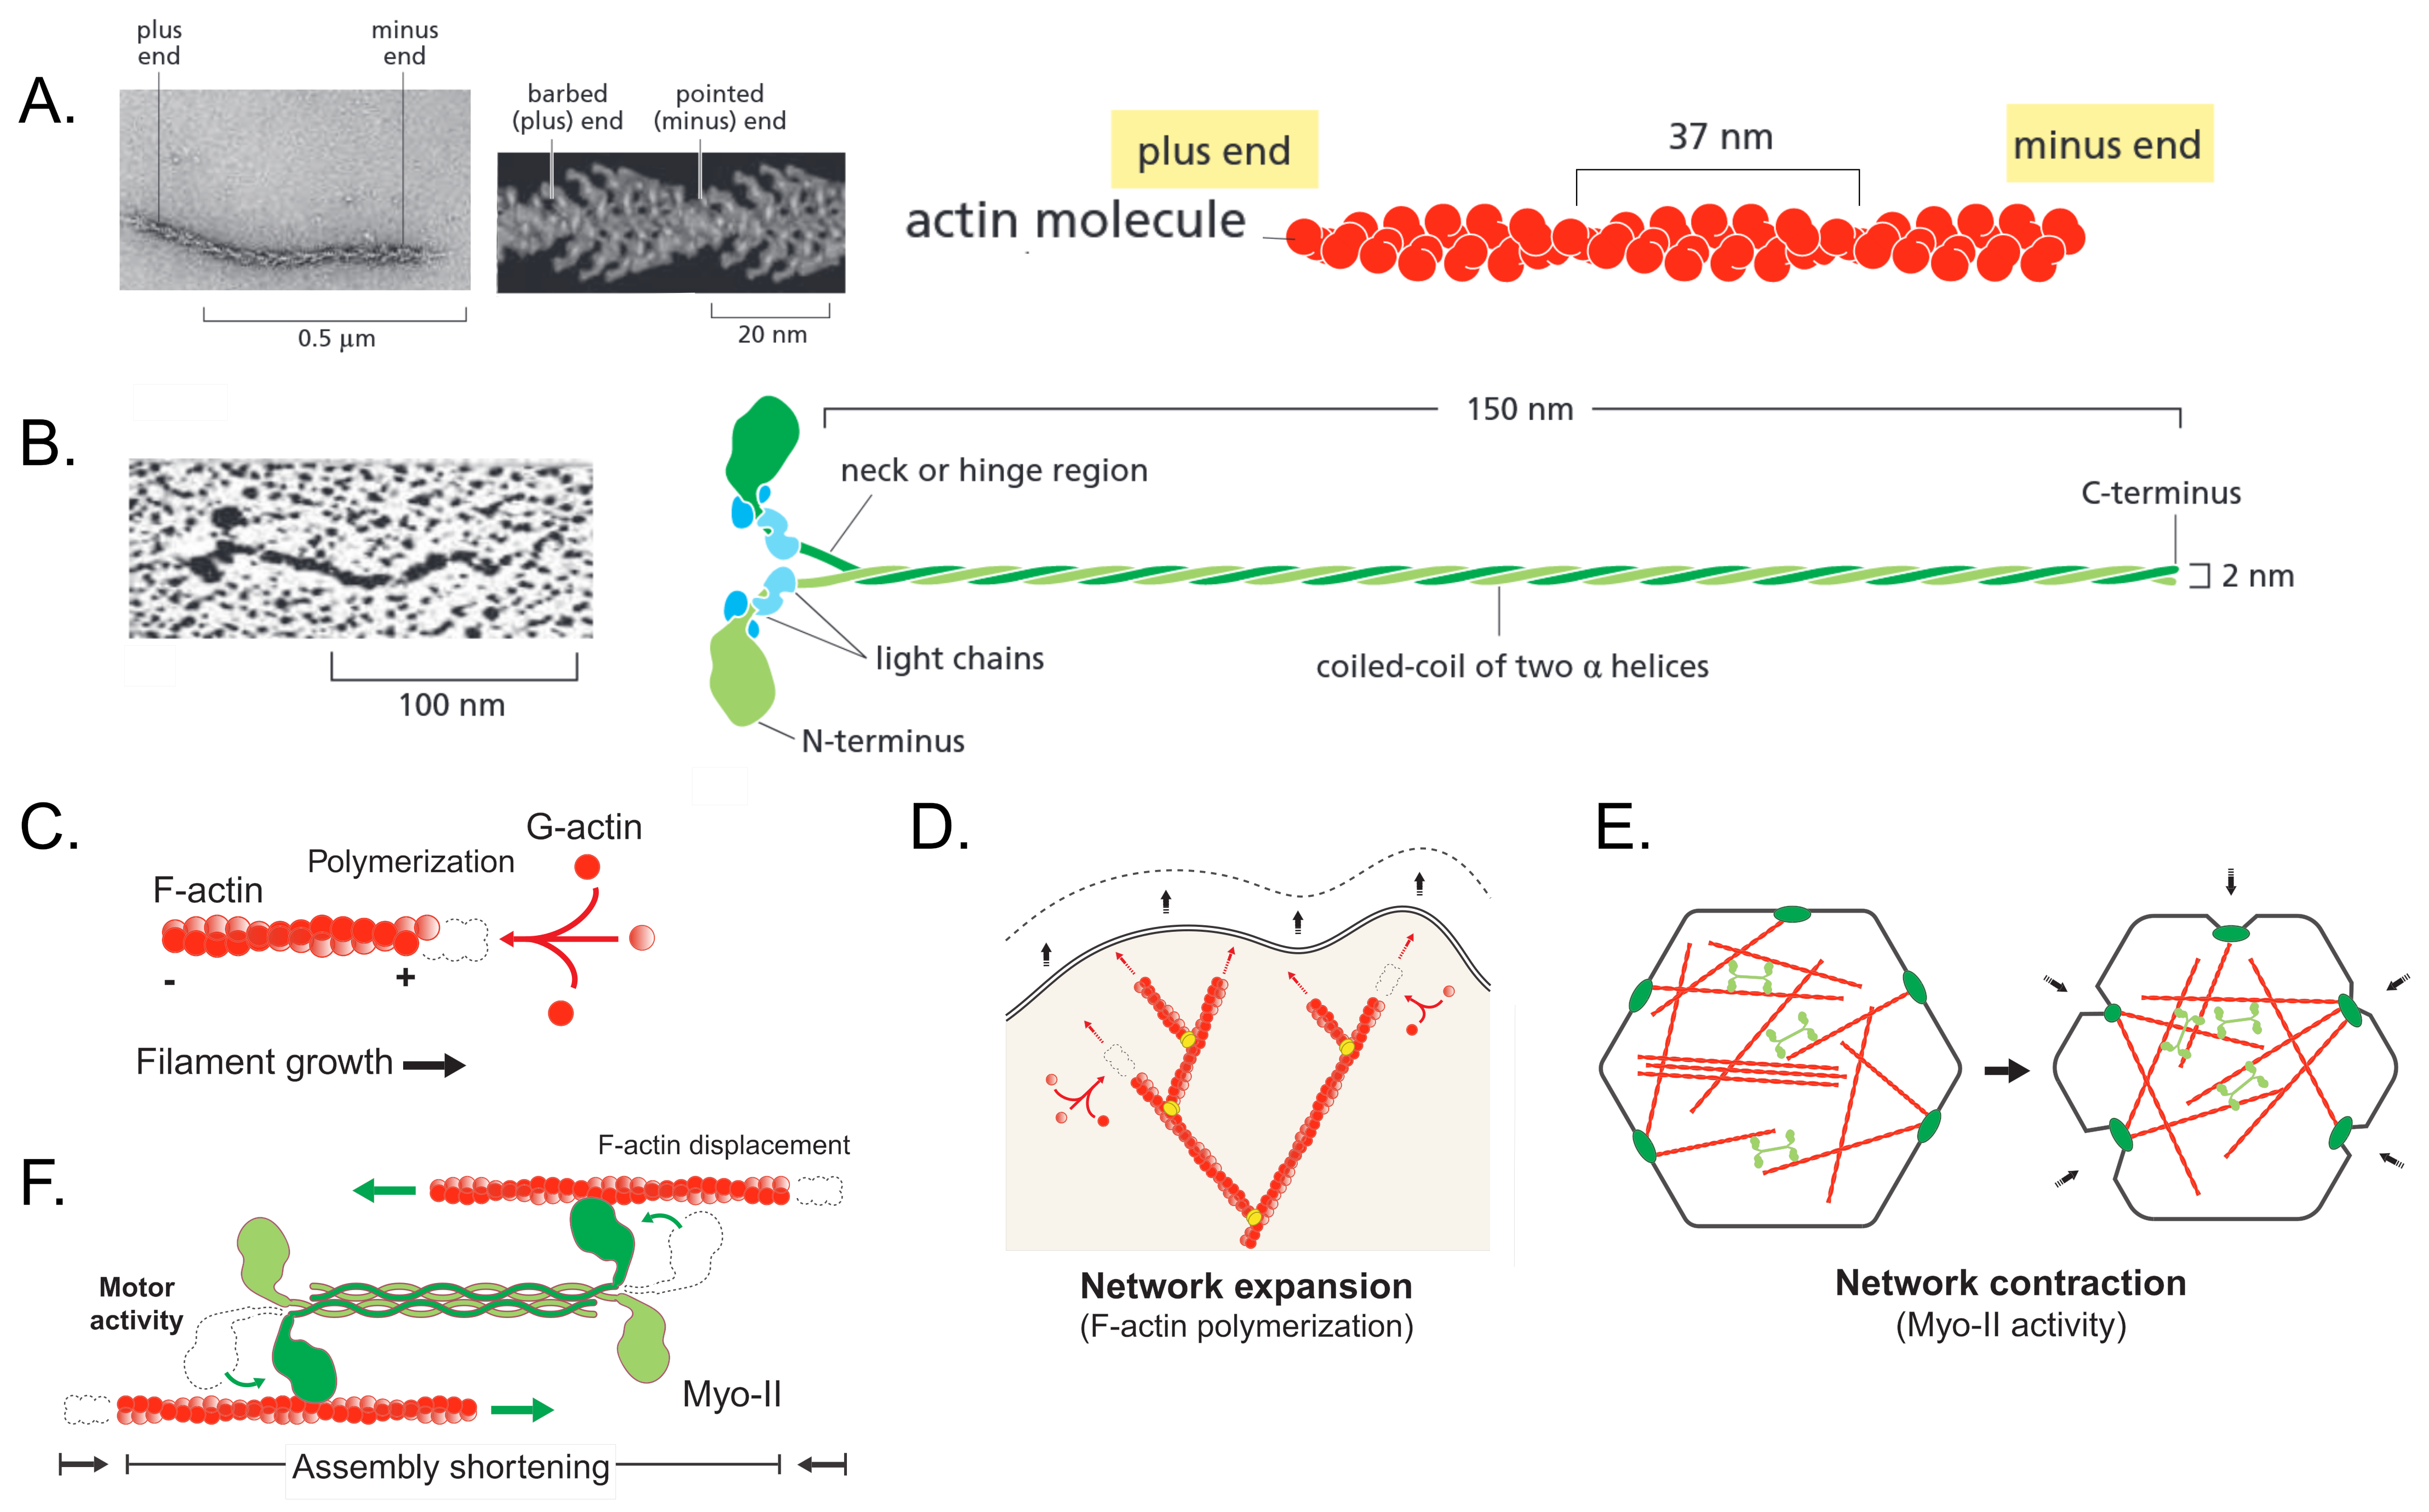
\includegraphics[width=\textwidth]{chap3actinmyosin.png}
	\caption{\label{fig_3_1} \textbf{Actin and Myosin}: (A) Electron micrograph of Actin filament with zoomed in images of barbed and pointed end. (B) Same for Myosin II minifilament with clearly visible two globular heads and a long tail. (C-D) Actin network can apply pushing force through polymerization of single filaments or network expansion. (E,F) While myosin activity would lead to contraction of the networks. \textit{Adapted from A-B \cite{alberts2015} and C-F \cite{clarke2021}}
	}
\end{figure}

\hypertarget{actin-networks}{%
	\subsection{Actin networks}\label{actin-networks}}

Actin filaments can also form branched networks, facilitated by the presence of nucleation sites on the filament and proteins containing actin-binding motifs. The actin nucleation can be catalyzed by two primary factors, the ARP 2/3 complex or formins. The ARP 2/3 complex creates a pointed end in the center of a filament, leading to the formation of a new branch from that site. This results in the formation of a tree-like network of branches, capable of generating sufficient pushing forces to move a part of the cell membrane (see Fig. \ref{fig_3_2} E,F). The formins, in conjunction with profilin, aid in the growth of the filaments, with profilin serving as a staging area for the rapid addition of monomers to the filament. These structures can take the form of dendritic actin networks that enable membrane protrusion at lamellipodia or spike-like projections of the plasma membrane that allow a cell to explore its environment (see Fig. \ref{fig_3_2} C). The pushing forces generated at the molecular level are of the order of 1 piconewton.


\begin{figure}[h!]
	\centering
	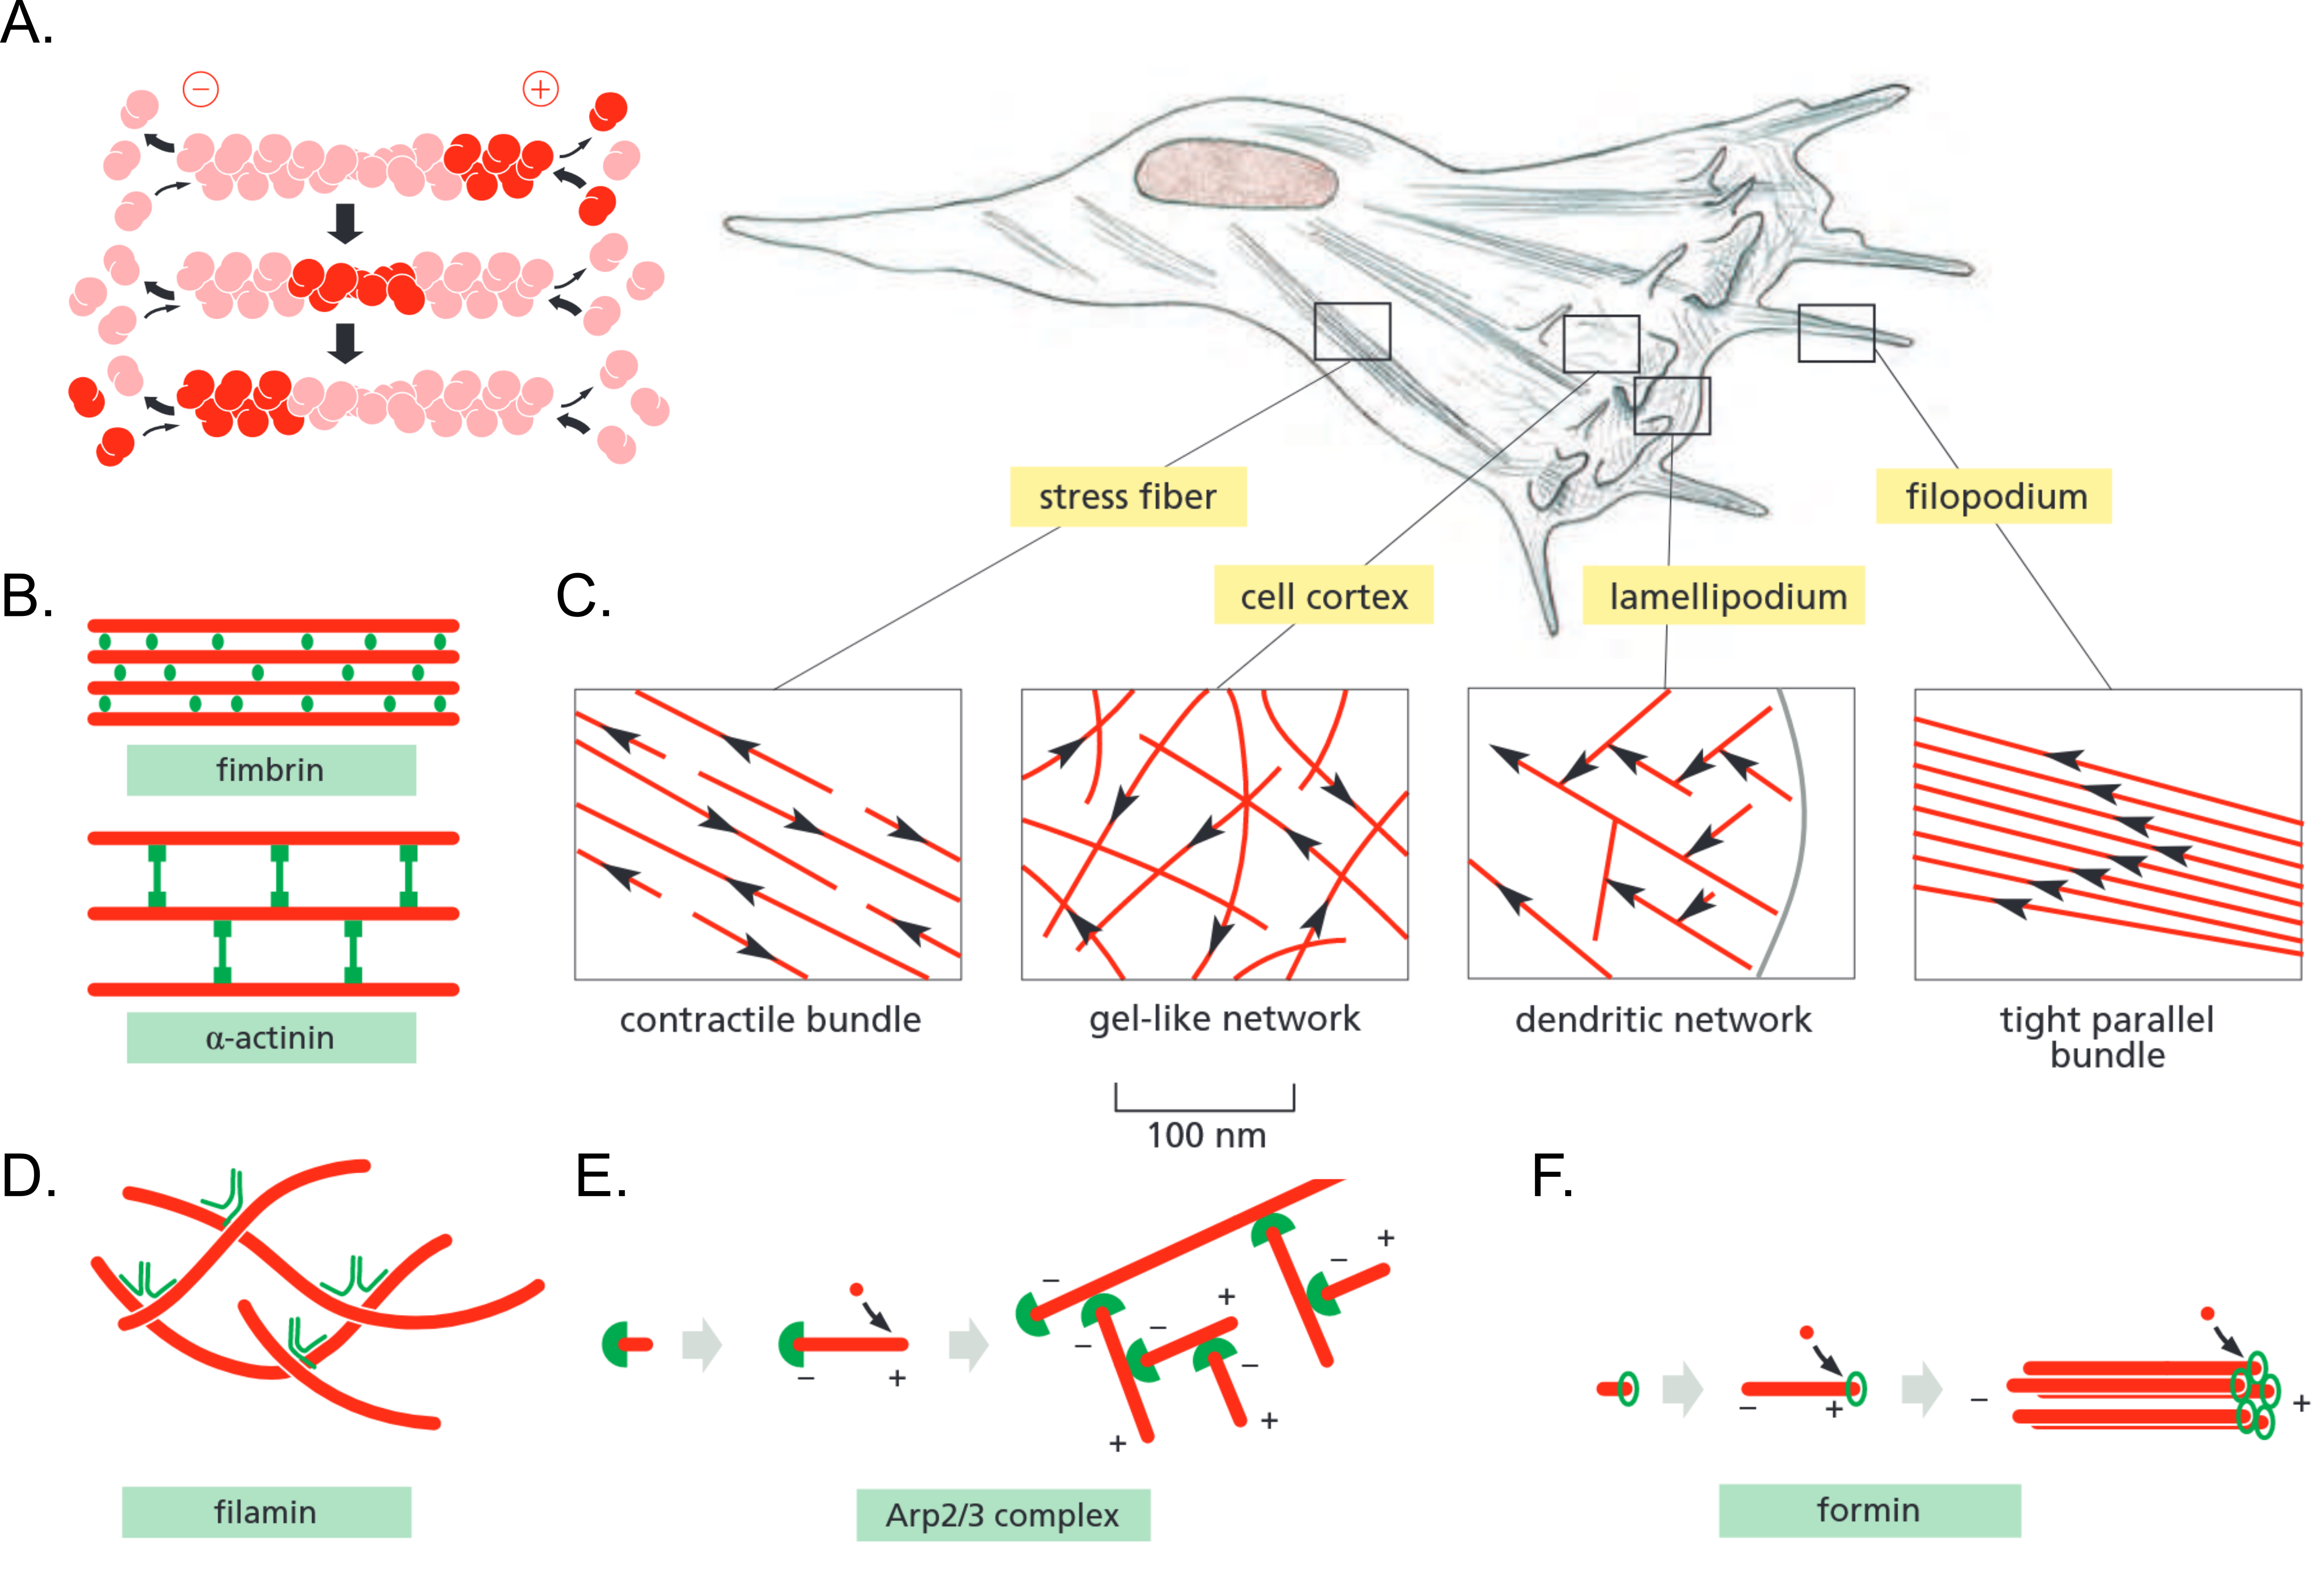
\includegraphics[width=\textwidth]{chap3actinstructures.png}
	\caption{\label{fig_3_2} \textbf{Forms of actin networks}: (A) Actin treadmilling: where highlighted actins move from positive end to negative end as the filament polymerizes and depolymerizes from both ends. (C) In an adherent cells, there are many different kinds of actin structures from contractile network to gel-like cortex. (B,D,E,F) Actin structures can be thought as meshwork of actin filaments (red) with crosslinkers(green). Different crosslinkers produce distinct form of actin network.  \textit{Adapted from \cite{alberts2015}}
	}
\end{figure}

\hypertarget{actin-cortex}{%
	\subsection{Actin cortex}\label{actin-cortex}}

The actin filaments can also form tight or loose bundles, facilitated by crosslinking proteins. Fimbrins enable multiple actin filaments to arrange in parallel, resulting in closely packed bundles that exclude myosin from connecting to the filaments. On the other hand, $\alpha$-actinin crosslinks actin filaments with opposite polarity into a loose bundle, allowing myosin to bind and create contractile bundles (see Fig. \ref{fig_3_2} B). Myosin II oligomerizes into a bipolar short filament that can connect multiple actin filaments and move across them, resulting in a pulling effect (see Fig. \ref{fig_3_1} B). This movement is driven by ATP hydrolysis making contracting an active process. The loose bundle forms the gel-like network in the cell cortex. Other actin crosslinking proteins can result in different structures. Filamin creates a loose and viscous gel that is essential for migration, while spectrin creates a strong and flexible web-like network of short actin filaments that allows cells to reversibly deform (see Fig. \ref{fig_3_2} D). The actomyosin bundles in the cortex can generate two orders of magnitude more force than a single filament \cite{clarke2021}.


\hypertarget{actin-structures-at-a-larger-scale}{%
\section{Actin structures at a larger scale}\label{actin-structures-at-a-larger-scale}}

During epithelial morphogenesis, individual cells can undergo shape changes by modifying their contractility or actin turnover, resulting in the development of tissue curvature. As mentioned previously, epithelial cells exhibit apicobasal polarity, which results in a non-uniform distribution of the actin cytoskeleton that influences cell shape and tissue architecture.

The geometry of columnar or wedge-like cells in a monolayer determines the specific ways in which they can be organized \cite{gomez-galvez2021}. Columnar cells, when arranged together, produce a flat tissue, while wedge-shaped cells with a narrow top result in convex curvature (see Fig. \ref{fig_3_4} A). Conversely, concave curvature with a narrow bottom can also be created. By observing the actin cytoskeleton, we can determine the specific mechanisms of tissue shaping (see Fig. \ref{fig_3_4} B). For example, apical constriction with concentrated actin cortex on the apical surface is involved in multiple convexly curved tissues, such as the invagination of the intestinal crypt, the Drosophila mesoderm, and the vertebrate lens placode \cite{perez-gonzalez2021, lecuit2011, houssin2020}.

\begin{figure}
	\centering
	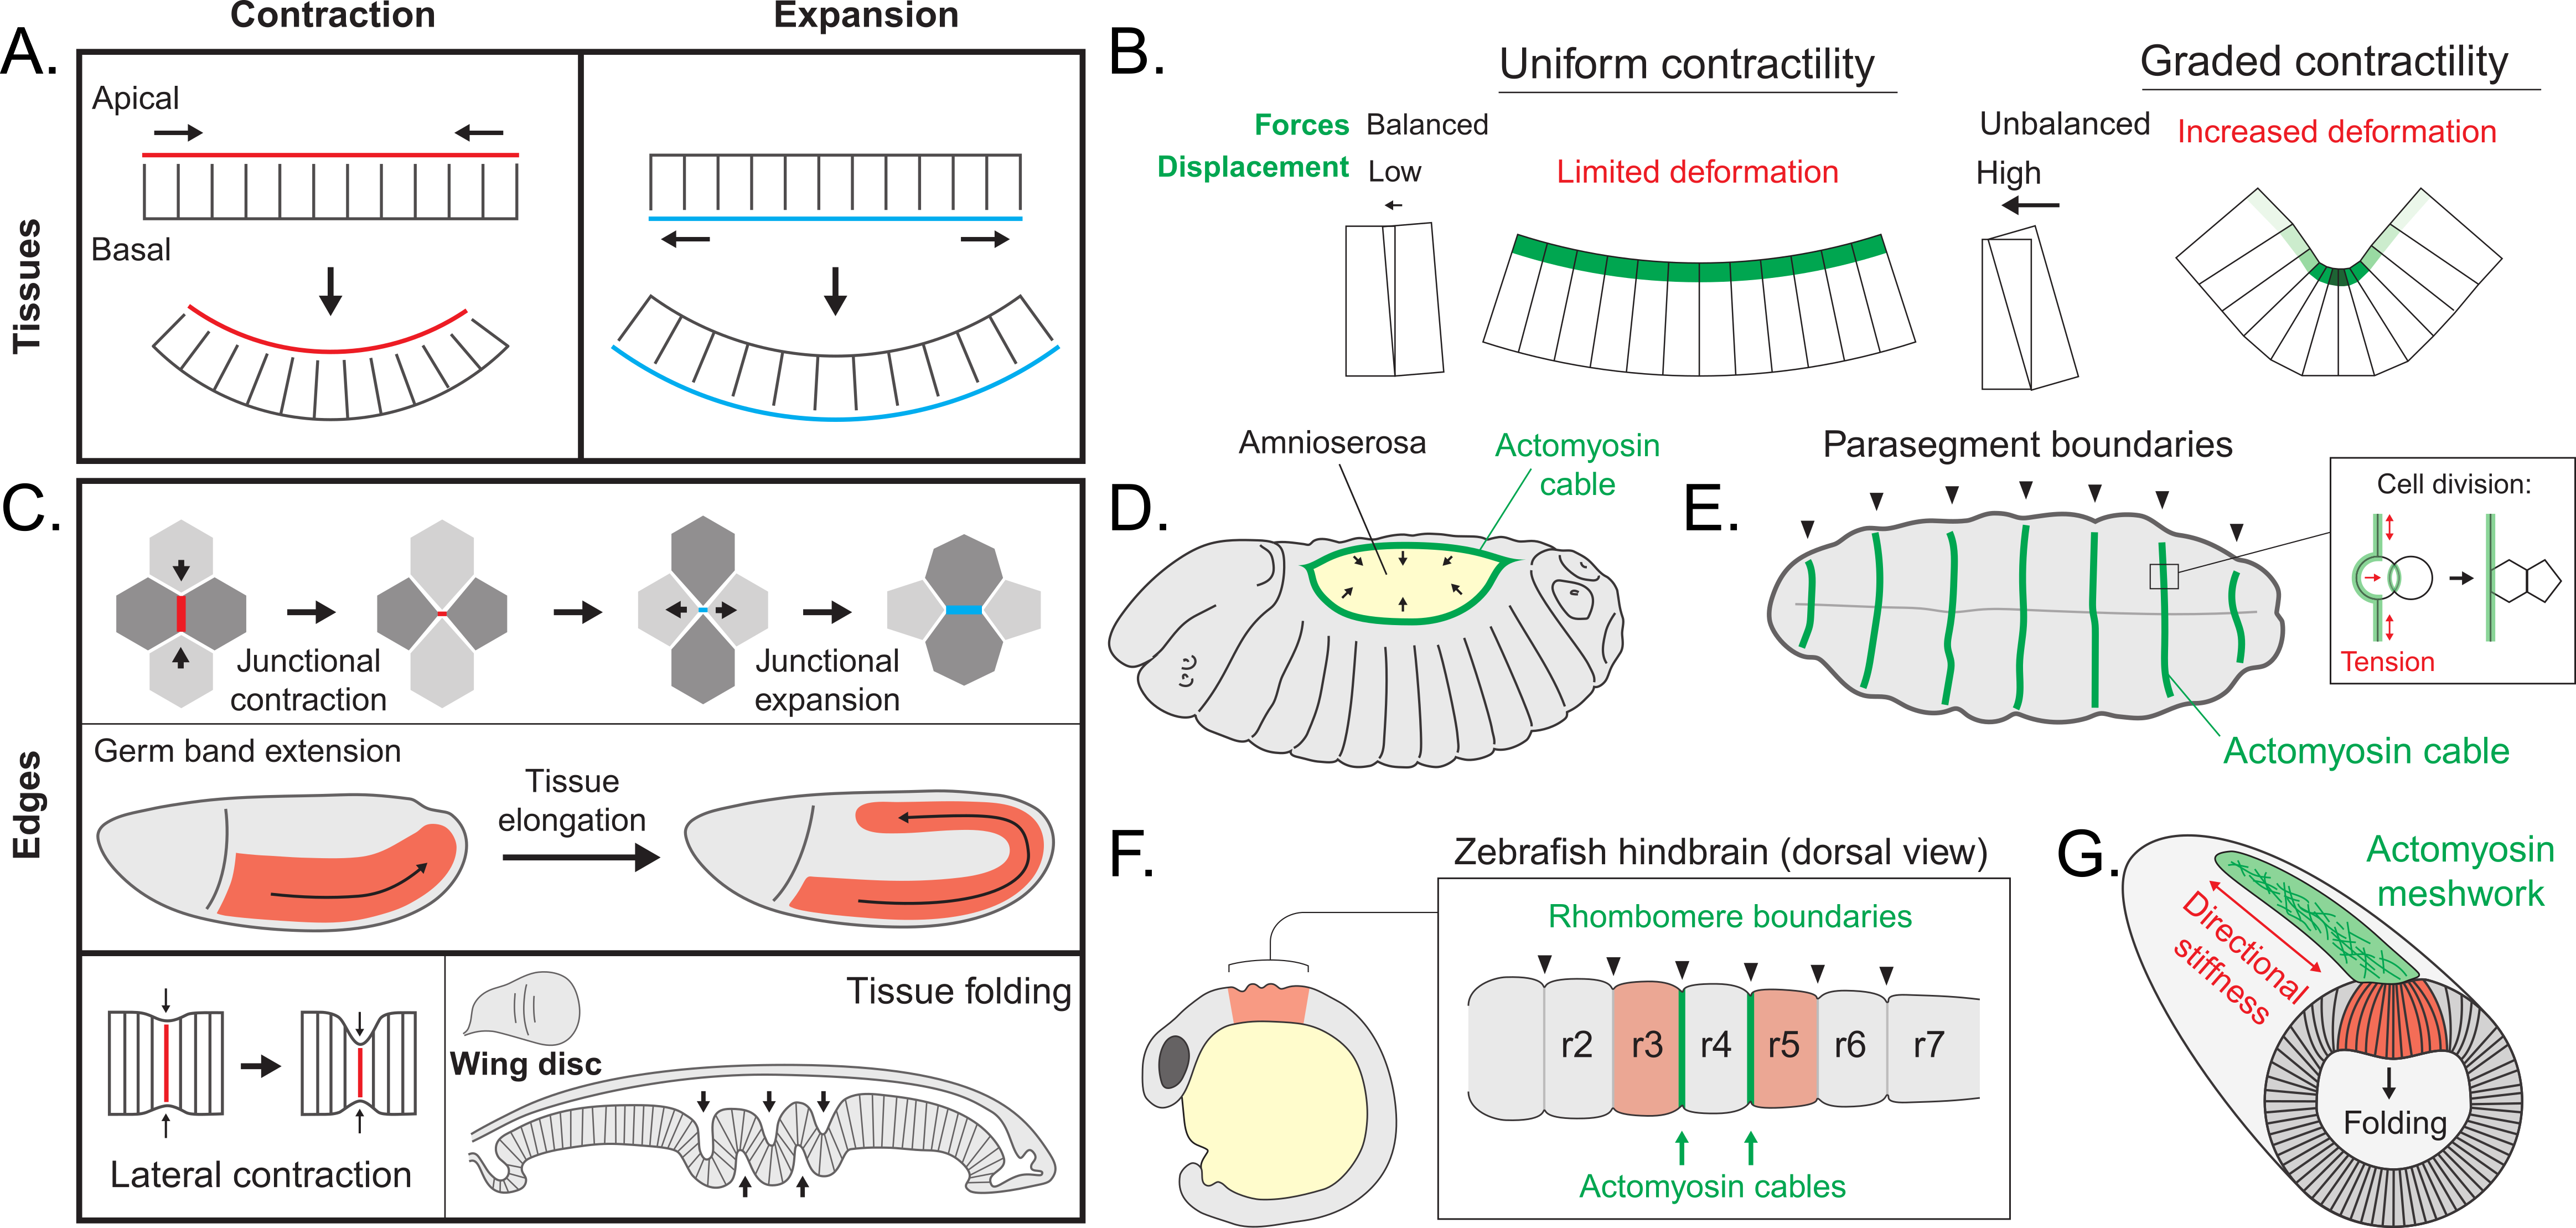
\includegraphics[width=\textwidth]{chap3actinsuper.png}
	\caption{\label{fig_3_4} \textbf{Morphogenesis driven by actin at tissue scale}: (A) Apical contraction or basal relaxation both results in the same curvature. (B) However, amount of deformation will depend on the contractility gradient. (C) Lateral surface of cells can also undergo expansion or contraction leading to cell rearrangements or tissue folding. (D-G) Supracellular actin cables plays vital role in creating boundaries or causing large scale deformations. \textit{Adapted from \cite{clarke2021}}
	}
\end{figure}

On the other hand, basal constriction results in opposite curvature, as observed in the optic cup and mid-hind brain fold of zebrafish \cite{sidhaye2017, gutzman2018}. However, convex curvature can also be produced through basal expansion, as seen in the Drosophila wing disc (see Fig. \ref{fig_3_4} A). Certain parts of the wing disc can locally relax the basal side without affecting the apical side, leading to basal expansion \cite{sui2018}. In addition to the apical and basal surfaces, lateral surfaces can also contract or expand due to myosin II activity, which can cause tissue folding in the wing and leg discs of Drosophila \cite{sui2018, monier2015}. Furthermore, cell-cell rearrangements can be produced by altering junction lengths during germ band extension \cite{yu2016, collinet2015} (see Fig. \ref{fig_3_4} C). 

Not only do individual cells undergo coordinated actin reorganization during epithelial morphogenesis, but supracellular actin structures can also emerge at the tissue level (see Fig. \ref{fig_3_3} A-C). Junctional actomyosin organizes to form bundles connected across multiple cells, allowing for important functions such as wound healing and morphogenesis \cite{brugues2014, clarke2021} (see Fig.~\ref{fig_3_4} D-F). These supracellular networks can exert forces at the scale of the embryo, as observed in cases such as dorsal closure and parasegment boundary formation in Drosophila and epiboly in zebrafish \cite{ducuing2016, calzolari2014}. Additionally, these networks can alter the material properties of specific regions in the embryo, making them more prone to deformation and thus aiding in the formation of folds or invaginations (see Fig. \ref{fig_3_4} G). 

During Drosophila gastrulation, tissue-level actin cortex is altered in the direction of the anterior-posterior axis, providing increased bending strength in that direction. This supports the internalization of the mesoderm by promoting folding in a perpendicular direction \cite{yevick2019}. Interestingly, highly organized actin bundles are also found in even larger systems such as Hydra, vertebrate smooth muscle, and the heart \cite{maroudas-sacks2021, palmer2021, cetera2014, helm2005} (see Fig. \ref{fig_3_3} D-F). These bundles assist in generating mechanical force patterns that create coordinated tissue movements at a global scale.

\begin{figure}
	\centering
	\includegraphics[width=\textwidth]{chap3realactin.png}
	\caption{\label{fig_3_3} \textbf{Actin organization at different scales}:(A) Electron micrograph of actin cortex of mitotic Hela cells \cite{kelkar2020}. (B) Different forms of actin organization in circular fibroblast cell \cite{jalal2019} Scale$= 10\mu m$. (C) Supracellular actin ring during wound closure \cite{brugues2014} Scale$=20 \mu m$. (D) Dorsal closure of amnioserosa with actin network \cite{ducuing2016} Scale$= 10 \mu m$. (E) Supra-cellular organization of actin for cellularization of coenocyte. Circle is $60 \mu m$ \cite{dudin2019}. (F) Hydra with actin network, whose nematic defects determines morphogenesis \cite{maroudas-sacks2021} Scale$= 100 \mu m$.
	}
\end{figure}

\hypertarget{timescales-of-the-actin-cytoskeleton}{%
	\section{Timescales of the actin
		cytoskeleton}\label{timescales-of-the-actin-cytoskeleton}}

Morphogenesis, the process of shaping and forming living structures, occurs at varying timescales and requires the cell cytoskeleton to change its shape accordingly. Rheological and mechanobiological experiments have given us insights into how cells respond to forces and deformations based on their magnitude and rate (see Fig. \ref{fig_3_5}; reviewed in \cite{wyatt2016}).

For fast deformations (in the range of milliseconds to seconds), cells exhibit predominantly elastic behavior, as there is insufficient time for the actin cortex to respond or remodel \cite{deng2006}. The cytoskeleton can store elastic energy and release it. At this scale, there is also flow of cytosol through the cortical mesh, resulting in poroelastic behavior \cite{moeendarbary2013}.

When forces or deformations are applied over longer timescales (seconds to minutes), cells exhibit an increasingly viscoelastic behavior \cite{kollmannsberger2011}. The actin cortex can flow and is unable to fully store energy. The actin filaments and crosslinkers, such as myosins and actinin, allow the cytoskeleton to remodel in response to mechanical perturbations through turnover in tens of seconds or a few seconds, respectively. Myosin mini filaments, however, can take longer to remodel, up to hundreds of seconds.

\begin{figure}[h!]
	\centering
	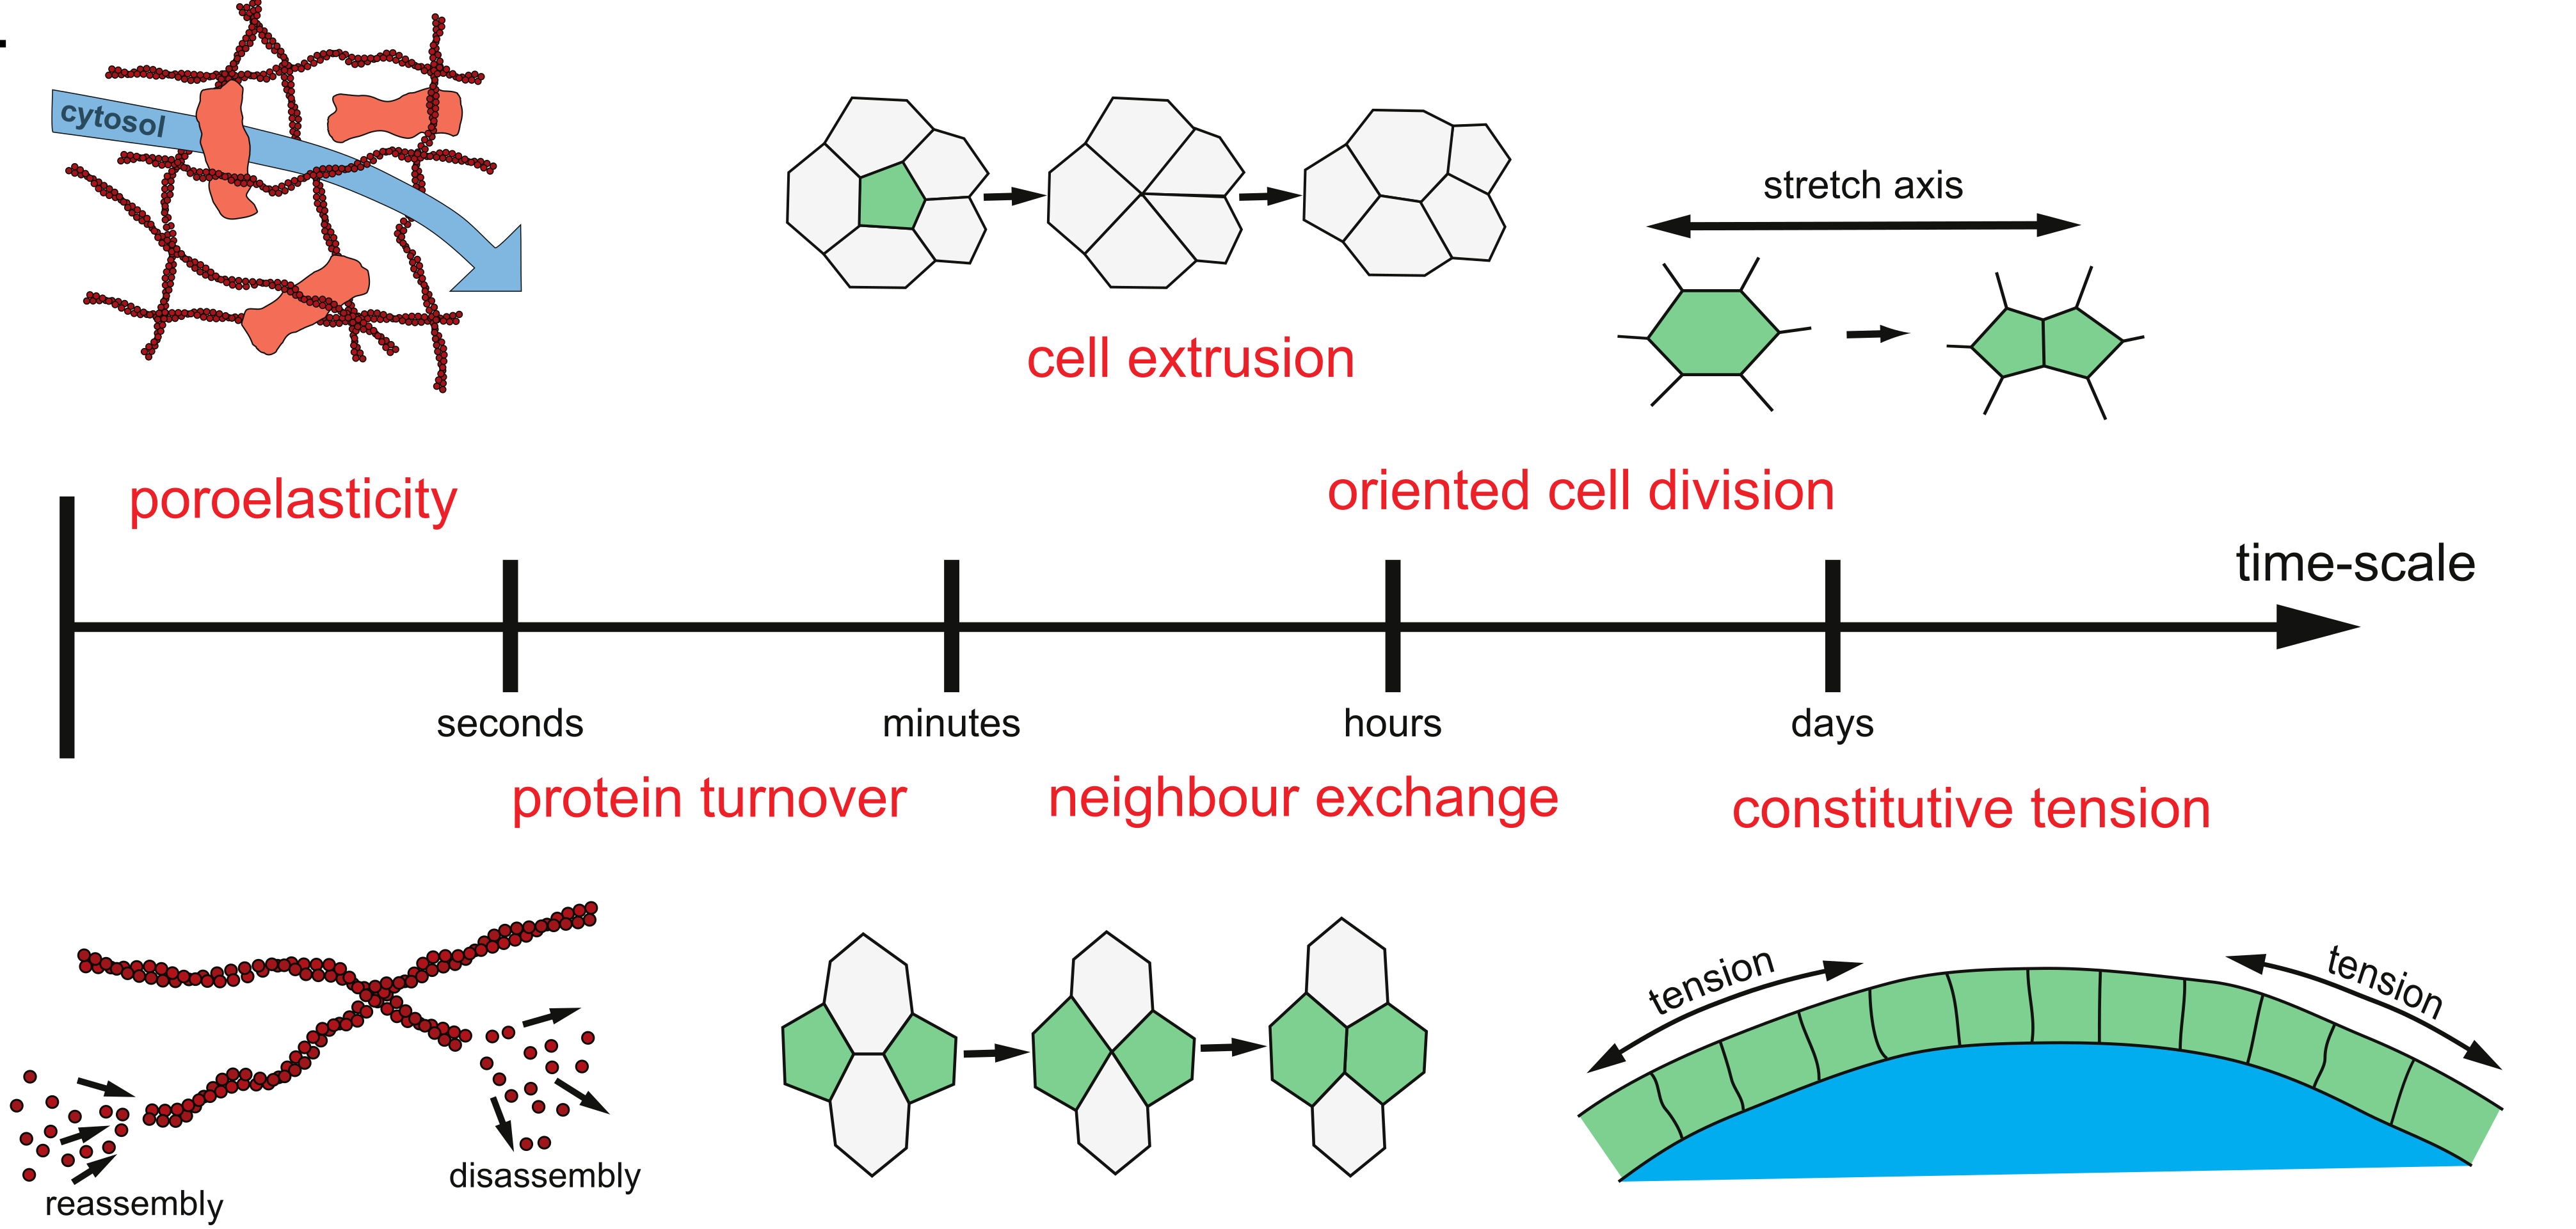
\includegraphics[width=\textwidth]{chap3timeactin2.png}
	\caption{\label{fig_3_5} 
		\textbf{Timescale of actin network related processes}: Timescales of different actin driven cellular processes, ranging from cytoskeletal fluid deformation to large-scale tissue deformations. \textit{Adapted from \cite{kelkar2020}}.}
	%\textbf{Molecular pathway and timescale of actin network related processes}: (A) Timescales of different actin driven cellular processes, ranging from cytoskeletal fluid deformation to large-scale tissue deformations. (B) Molecular signaling of RhoGTPase. RhoGEFs return GDP for GTP to activate RhoA. In turn RhoA results in actomyosin contractility. \textit{Adapted from \cite{kelkar2020, wyatt2016}}.
\end{figure}

At even longer timescales (minutes to hours), cells or tissues may respond through oriented division or rearrangement, allowing them to adapt to persistent forces such as gravity or surface tension. Tissues may resemble a viscous fluid and morph into a sphere, such as a blastocyst. Interactions with the extracellular matrix over hours can lead to adjustments in the constitutive tension of tissues based on biophysical and biochemical forces \cite{porazinski2015}.


%\hypertarget{controlling-cortical-tension}{%
%	\section{Controlling cortical
%		tension}\label{controlling-cortical-tension}}
%
%The magnitude of contractile or tensile forces exerted by cells is greatly influenced by the tissue type and its environment. The signaling pathways regulating the crosslinkers and nucleators of actin bundles are responsive to both external biochemical and biomechanical stimuli (see fig \ref{fig_3_5} B; reviewed by \cite{kelkar2020}). The actomyosin bundles, made up of dynamic actin filaments, constantly undergo cycles of contraction, polymerization, and depolymerization, which maintain a homeostatic level of cortical tension in healthy tissues. As a result of the numerous components involved in the actin network, cortical tension can be readily modulated by pharmacological interventions targeting specific molecular targets \cite{cartagena-rivera2016}.
%
%For example, the use of Latrunculin, which binds to actin monomers, can result in the depolymerization of the actin network and reduce contractility. Similarly, inhibiting myosin activity with Blebbistatin leads to a decrease in cortical tension due to its hindrance of myosin II ATPase activity. Conversely, Calyculin-A enhances contractility by accelerating the rate of Myosin II phosphorylation. The stability of the actin network can also be impacted by sequestering ARP 2/3 monomers with CK666, which increases cortical tension. Other factors, such as Rho-GTPases and calcium levels, located further along the signaling pathway, can also affect network stability \cite{valon2017}.
%
%Optogenetic tools offer a more refined and localized means of controlling contractility. For instance, tools based on the regulation of RhoA can be used to locally regulate cell protrusion, tissue tension, and traction \cite{valon2017}. A recently developed tool controlling Shroom3 provides even finer control over apical constriction and can be used to recreate tissue folding \cite{martinez-ara2022}.

\hypertarget{modeling-active-tissue-dynamics}{%
	\section{Modeling active tissue
		dynamics}\label{modeling-active-tissue-dynamics}}

The advancement of molecular biology and tissue dynamics has increased our understanding of morphogenesis. However, it is becoming increasingly crucial to interpret biological experiments through theoretical models in order to generate new hypotheses and validate them through further experimentation.

Mathematical models at multiple scales are used to describe both physics and biology. At larger tissue scales, hyperelastic continuum material models could be utilized to describe the behavior of the cardiovascular system \cite{holzapfel2019}. On smaller scales, agent-based models are used to explain epithelial tissue behavior in terms of cell sorting and reorganization \cite{voss-bohme2012}. This section aims to provide the reader with a brief overview of the relevant modeling approaches in this field.

\hypertarget{vertex-models}{%
	\subsection{Vertex models}\label{vertex-models}}

D'Arcy Thompson, in his chapter on ``The Forms of Tissues,'' presents an intuitive argument regarding the role of surface tension or capillarity in organizing cells into a tissue \cite{thompson1979, graner2017}. He observed this phenomenon in a wide range of biological systems, from two connected cells to the organization of cells in a dragonfly wing, which resemble the
associations of soap bubbles or foams (see Fig. \ref{fig_3_6}).\footnote{"we recognize the appearance of a "froth," precisely resembling that which we can construct by imprisoning a mass of soap-bubbles in a narrow vessel with flat sides of glass; in both cases we see the cell-walls everywhere meeting, by threes, at angles of $120 \deg$, irrespective of the size of the individual cells: whose relative size, on the other hand, determines the curvature of the partition-walls", writes Thompson}
In the case of monolayered epithelial tissue, its polygonal cellular pattern on its surface enables the easy description and tracking of cell motion and shape change through the use of vertices and edges.

\begin{figure}
	\centering
	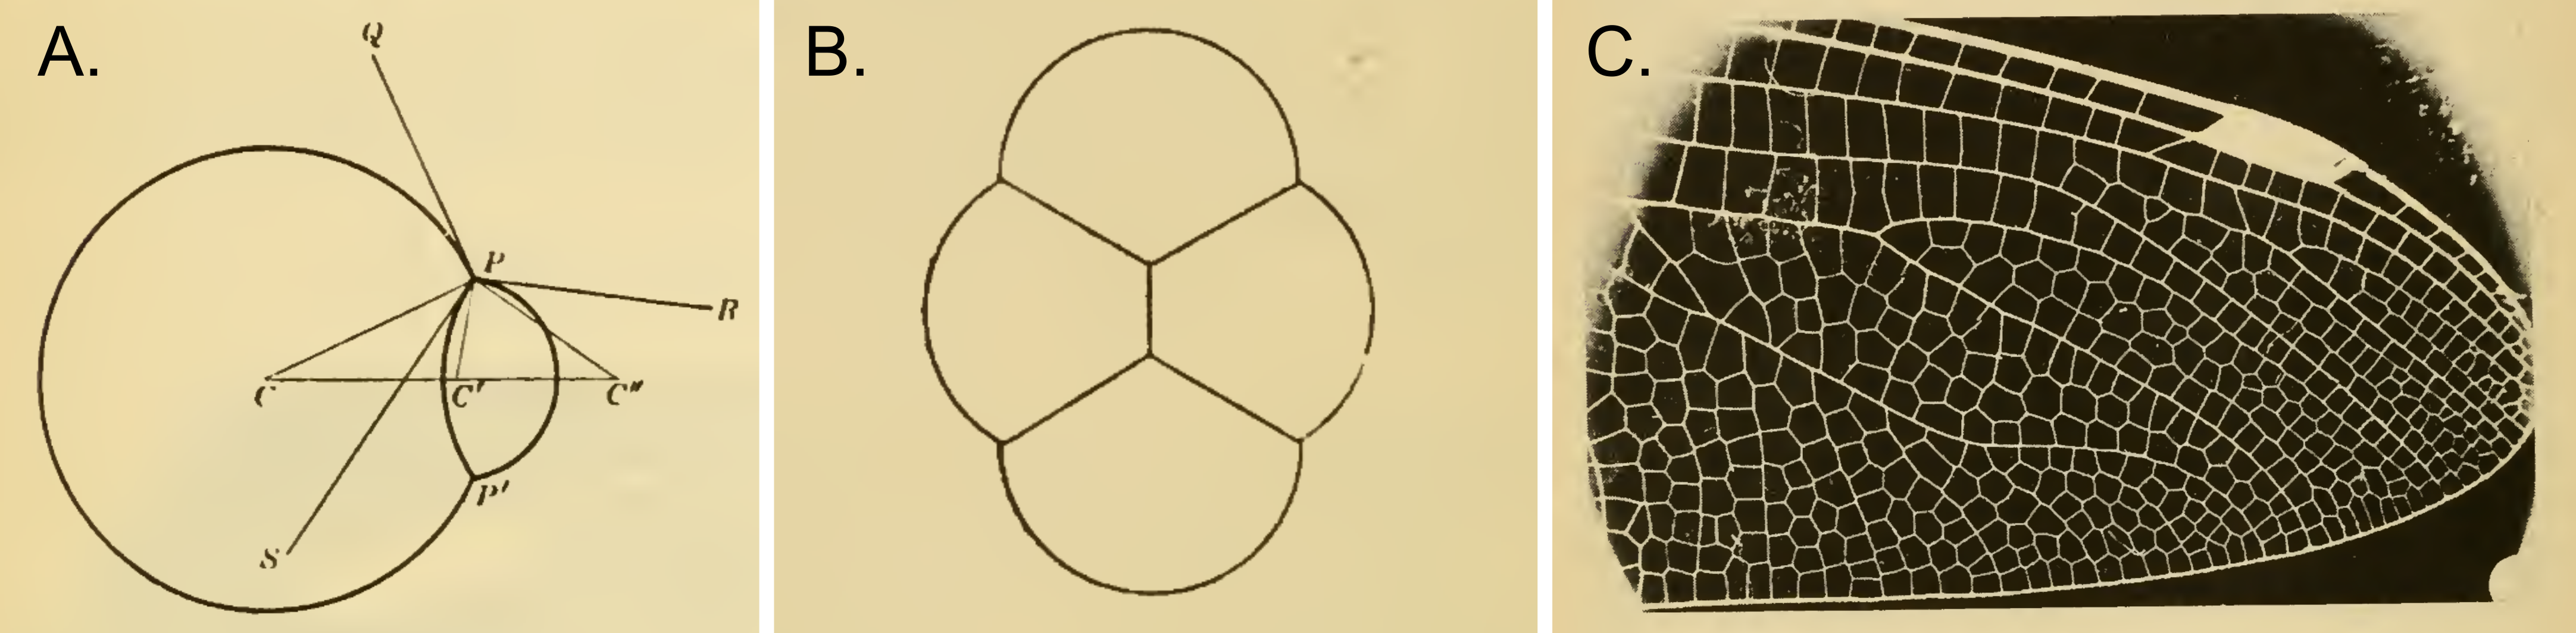
\includegraphics[width=\textwidth]{chap3darcy.png}
	\caption{\label{fig_3_6} \textbf{D'Arcy Thompson's forms of tissues:} (A-B) Thompson equates cell aggregates to coalescence of bubbles like in a froth. (C) A dragon fly wing is a clear example of this organization. \textit{Adapted from \cite{thompson1979}}
	}
\end{figure}

Vertex models have proven to be valuable in understanding the complex interactions between cellular shape, the forces generated within epithelial cells, and the mechanical constraints imposed on the tissue from external sources (as reviewed in \cite{alt2017}). These models can be two-dimensional or three-dimensional, depending on the system being modeled, but cells are consistently defined as having both an apical and basal surface, as well as lateral interfaces between neighbors. Further complexities have been added to describe specific systems, such as intercalations in three-dimensional epithelia, through the use of a geometric shape known as the Scutoid (reviewed in \cite{gomez-galvez2021}).

\begin{wrapfigure}{r}{5.5cm}
	\caption{\textbf{Vertex model for cells in a monolayer} \textit{Adapted from \cite{gomez-gonzalez2020}}.}\label{fig_3_7}
	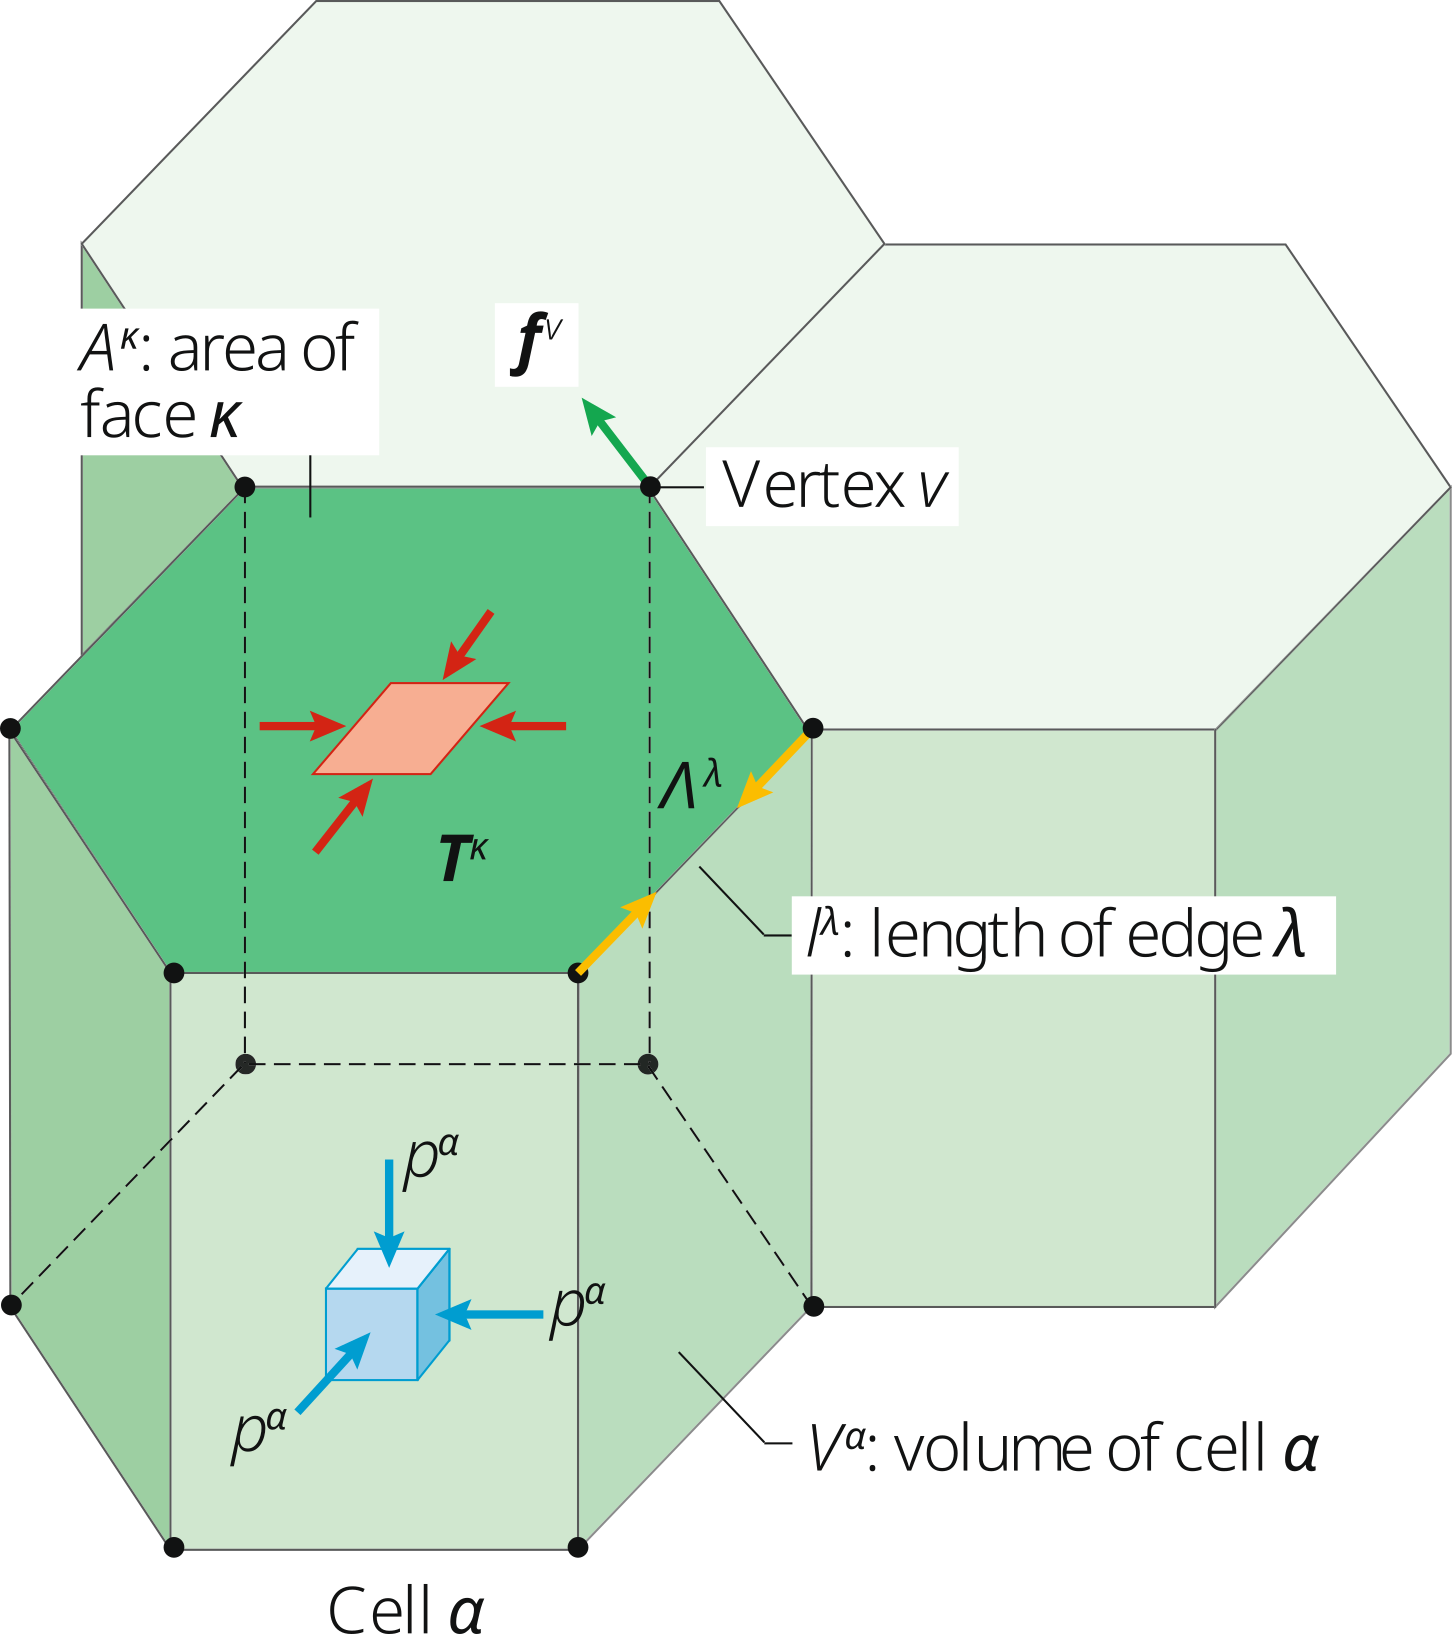
\includegraphics[width=5.5cm]{chap3vertex.png}
\end{wrapfigure} 

To determine the motion of the vertex, mechanics must be specified. It is often done using the virtual work function (W). There are two components: internal $(\delta W_i)$ and external $(\delta W_e)$. 
$$ \delta W = \delta W_i + \delta W_e .$$ 
The changes in internal virtual work,  $(\delta W_i)$ can result from changes in the cell volumes $(\delta V)$, in the areas of surfaces $(\delta A)$, or in the lengths of bonds $(\delta l)$. By defining the cell pressure $(P)$, the surface tension $(T)$, the line tensions $(\Lambda)$, and internal dissipative forces $(f_i)$, the differential of the internal virtual work for vertex movements can be written. 
$$ \delta W_i = \Sigma_{cell\ \alpha} \left( -P^\alpha \delta V^\alpha \right) + \Sigma_{surface\ k} \left( T^k \delta A^k \right) + \Sigma_{edge\ \lambda} \left( \Lambda^\lambda \delta l^\lambda \right) - \Sigma_{vertex\ \nu} \left( f_i^\nu \delta x^\nu \right). $$
Similarly, the external virtual work, $(\delta W_e)$, can be written according to the external forces $(f_e)$ that come from external mechanical forces applied to the tissue through the matrix, or fluid pressure acting on apical or basal cell surfaces.
$$ \delta W_e =  - \Sigma_{vertex\ \nu} \left( f_e^\nu \delta x^\nu \right). $$

The state of a monolayer is determined by minimizing the virtual work function, taking into account the molecular complexities that contribute to surface tension and line tensions. In the context of epithelial layers, the actin cortex significantly impacts the tensions along the edges. Vertex model simulations in 2D models demonstrate the important role of interfacial tensions in shaping cell orientation, coordinating collective migration, and facilitating tissue rearrangement through cell division.

In contrast, 3D models capture the physics of various morphogenetic processes, such as the formation of appendages on the drosophila eggshell and the mechanical compartmentalization of intestinal epithelia \cite{osterfield2017, perez-gonzalez2021}. These models offer unique insights into cell packing and the transition between jamming and unjamming \cite{park2015, tang2022}. In some cases, phase transitions from a solid to fluid state result from localized proliferation and oriented divisions, showing that the epithelial tissue behaves as an active material (reviewed in \cite{lenne2022}).

\hypertarget{continuum-models}{%
	\subsection{Continuum models}\label{continuum-models}}

The viscoelastic properties of tissues are captured in vertex models, which are useful for smaller scale. However, for larger scale deformations or flows, we can model tissues as a continuous material. There are two tactics for thinking about these models: one focuses on the rheological properties of the tissue, and the other on shape transformations. By thinking of a continuous sheet of cells as an active surface, we can capture the physics of single cells to embryos \cite{salbreux2017, khoromskaia2023}.

Continuum models focus on developing reliable constitutive relations and solving initial-boundary-value problems. Constitutive relations describe how materials respond to applied loads, and they depend on the internal constitution of the material. Determining constitutive relations for epithelial monolayers can be challenging because these tissues are much more complex than simple metals or passive polymers (see Fig. \ref{fig_3_8} A-B). However, their complex material behavior can be understood by characterizing their mechanical response using standard material testing techniques \cite{humphrey2002}. Typically, they can be probed mechanically in a biologically relevant manner, such as through biaxial or uniaxial stretching experiments that simulate \textit{in vivo} tissue behavior \cite{humphrey2014}. These experiments with epithelial tissues have revealed the viscoelastic nature of these materials \cite{harris2012, khalilgharibi2019}.

Solids, such as rubber, are considered to have elastic properties, allowing them to deform reversibly when subjected to a force. Conversely, fluids are characterized by their viscosity, meaning they flow in response to an applied force. Viscoelastic materials exhibit both solid-like and fluid-like behaviors (see Fig. \ref{fig_3_8} C). Simple models can represent these behaviors by combining elastic components, represented as springs, and viscous components, represented as dashpots. The elastic response does not dissipate energy, unlike the viscous response. $$ \sigma = E\epsilon ,\ \ \ \ \sigma = \eta \frac{d\gamma}{dt}. $$ Other material properties like stiffness or Poisson's ratio can be revealed through quasi-static stretching or compression. However, dynamic properties are better understood through frequency sweep, creep, or stress relaxation experiments \cite{guimaraes2020}. Rheological experiments have been extremely valuable in gaining insight into the mechanical response of various biological materials, ranging from reconstituted cytoskeletal proteins to large multicellular aggregates \cite{mofrad2009, cavanaugh2020, xi2018}.

Rheological properties are often linked to physiological state and are crucial for their specific functions \cite{park2015, vedula2012}. For example, many fundamental shape transitions in embryos occur through abrupt change in tissue material properties \cite{hannezo2022}. Therefore, it is important to assess rheological properties in different microenvironments. Mechanical information such as deformation, deformation rates or velocity fields, traction forces exerted by cells on substrates, and intercellular mechanical stress can provide a more complete picture of tissue rheology when combined with information about cellular architecture obtained through imaging \cite{roca-cusachs2017}. These types of experiments shed light on the complex mechanisms of strain stiffening and viscoelastic behavior at different deformation regimes involving various parts of the cytoskeleton.

\begin{figure}
	\centering
	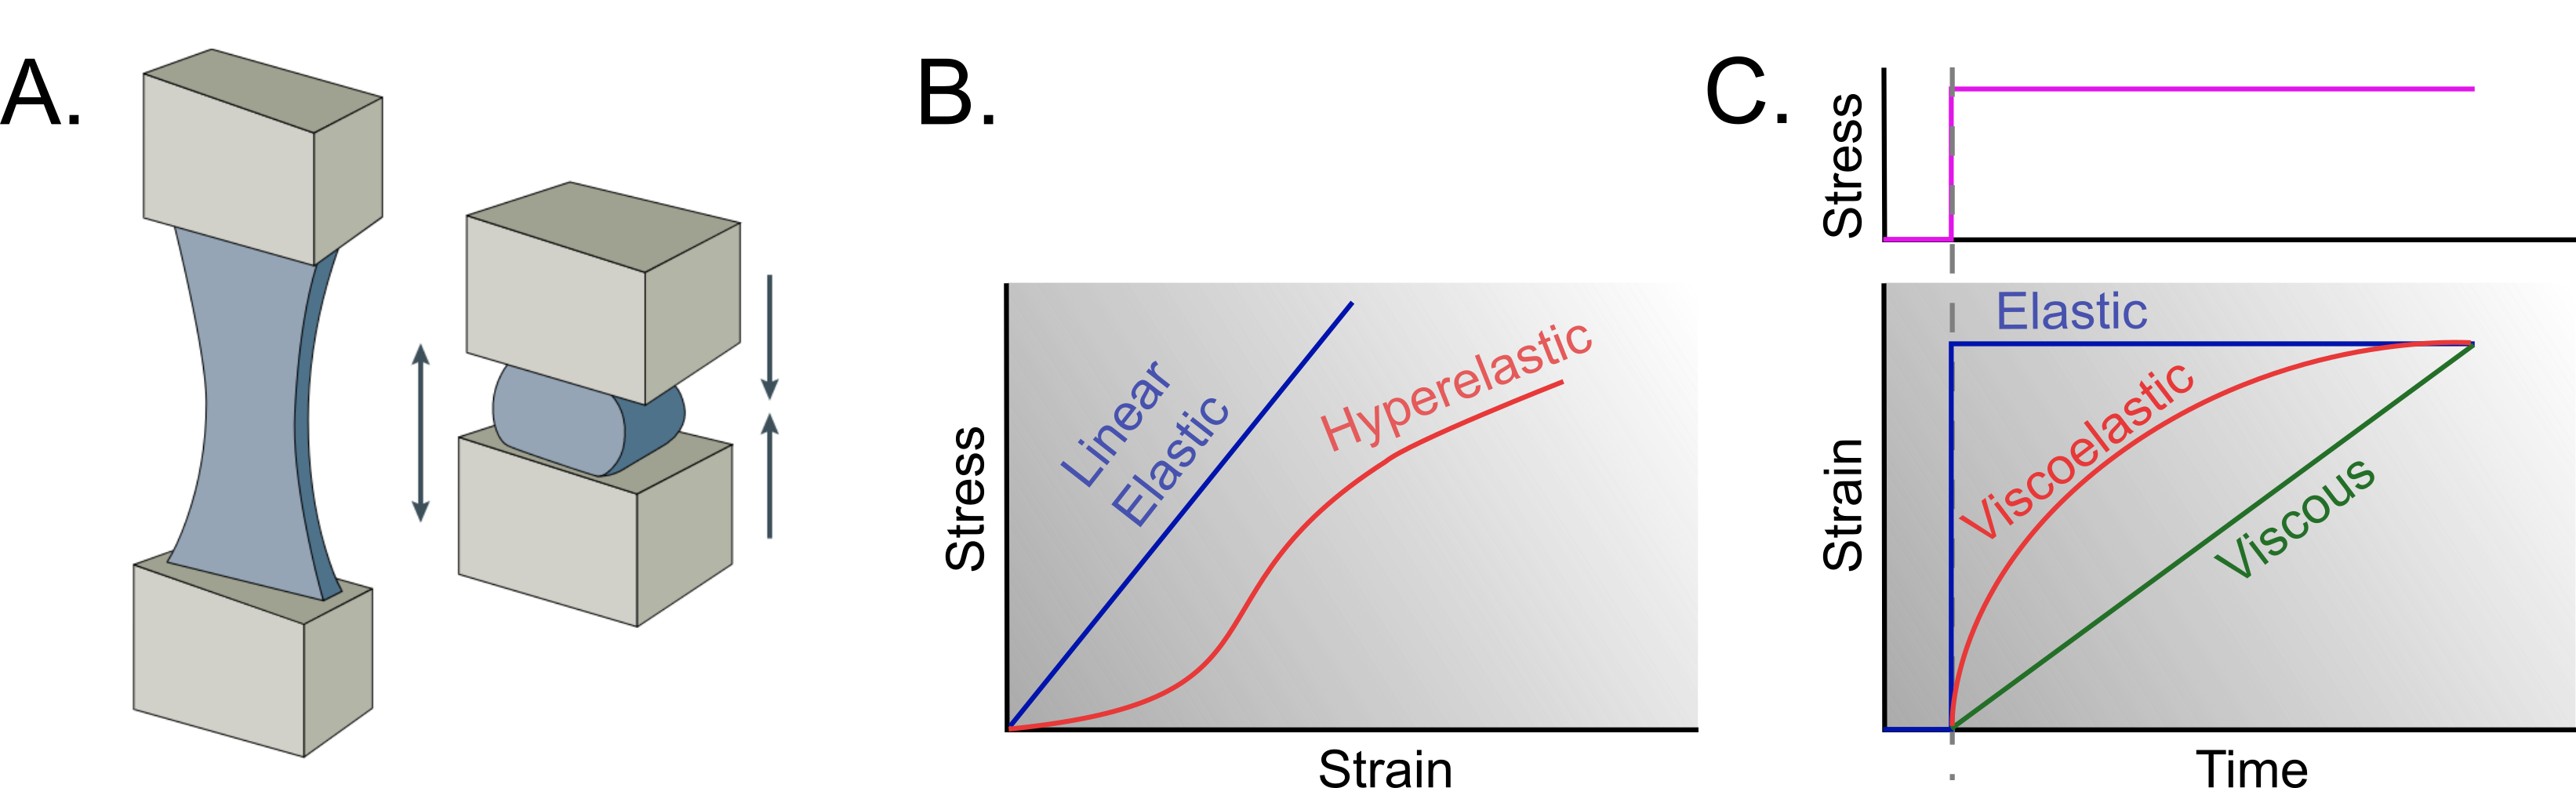
\includegraphics[width=0.85\textwidth]{chap3elastic.png}
	\caption{\label{fig_3_8} \textbf{Stress strain behavior of materials}: (A) materials being stretched or compressed. (B) Quasistatic deformations yield stress-strain curves. (C) Creep test where strain response is characterized at constant stress.
	}
\end{figure}

One general feature of most biological tissues is their softness, and hence the fact that they undergo large deformations. However, linear elasticity is valid for infinitesimally small deformations. To account for such large deformations, geometrically exact continuum mechanics descriptions have been applied to a variety of systems including cardiovascular mechanics or the growth of organs. In this approach, deformation is described by a function  \(x = \chi (X, t)\) mapping a reference to a deformed configuration. The deformation gradient and Green's strain tensor (nonlinear in the deformation) are defined as
$$ F = \nabla_X \chi(X, t);\ \ \ \ E = \frac{1}{2}(F^T F - I). $$ 
Based on these deformation measures, hyperelasticity is based on defining a strain energy function $W(E)$ from which elastic stresses can be computed as $S = {\partial W}/{\partial E}$. 


%However, in certain cases like modeling cardiovascular mechanics or the growth of organs, we can rely on hyperelasticity or composite material framework \marino{[what is this composite material framework? I edit a bit the following paragraphs]}. The basic kinematics assumes a mapping, \(x = \chi (X, t)\), deformation from reference to deformed configuration. The deformation gradient and Green's strain tensor are defined. 
%$$ F = \nabla_X (\chi(X, t)));\ \ \ \ E = \frac{(F^T F - I)}{2}. $$ 
%The elastic and growth can be delineated in the deformation gradient through decomposition. \[ F = F_e F_g .\] Here, in the theoretical framework of finite elasticity, one can assume a strain energy function relates to stress. The stress-strain data extracted from the experiment allows for predicting the form of the strain energy function. \[ S = \frac{\delta W}{\delta E}.\]

The use of hyperelastic models has proven to be effective in capturing the material response in various biological tissues, such as the bladder, heart tissue, skin, and arteries \cite{holzapfel2000}. This type of formulation provides a degree of flexibility, as it allows for the inclusion of additional physical constraints, such as the anisotropy of the tissue microstructure or its incompressibility. Minor modifications to these constitutive relations can be used to capture the material response, such as explaining the phenomenon of strain stiffening, or accounting for the inhomogeneity in the material, such as the collagen content and crosslinking in the tissue \cite{holzapfel2019}.

These models are also employed in the understanding of growth and remodeling, by expanding the framework of hyperelasticity through the use of kinematical growth theory \cite{ambrosi2019}. In such theories, the deformation gradient is decomposed into elastic and growth components $F = F_e F_g$, with the stress depending on the elastic part of the deformation gradient and $F_g$ being determined by a growth law. This theory highlights the existence of residual stresses in growing tissues, leading to a modification of the tissue properties into a spatially inhomogeneous and anisotropic states. This process is of great significance in the field of solid tumor growth mechanobiology, as the residual stresses directly impact tumor aggressiveness, nutrient pathways, necrosis, and angiogenesis.

\hypertarget{active-surface-models}{%
	\subsection{Active surface models}\label{active-surface-models}}

At the cellular level, the mechanical properties of tissues are largely determined by the biopolymeric cytoskeleton, which consists of filaments and cross-linkers and molecular motors. These components continuously convert energy, ATP to ADP, through contractions or extensions of the network, resulting in a physical gel-like system due to its cross-linked actin filament network. However, the presence of phenomena such as treadmilling, active polymerization-depolymerization of filaments, and the mobility of molecular motors, such as myosin, makes the tissue system an active gel that lacks time-reversal symmetry due to its continuous energy transduction.

Additionally, the filaments are polar, which allows for the acquisition of orientational order. This has led to the modeling of tissues as active gels, similar to modeling active systems, such as flocks of birds and schools of fish, using hydrodynamics of active matter \cite{julicher2018}. Active matter systems are a subclass of continuum models used to describe the dynamics of packed active particles, which are based on the liquid crystal theories of soft condensed matter. Like liquid crystals, cells also possess orientation and the ability to move past each other. In this framework, the orientation of filaments in the cytoskeleton or the elongation of cells in the tissue can be characterized by a nematic order parameter matrix (see Fig. \ref{fig_3_10}).
$$Q = \frac{3S}{2}\left(n\otimes n  -       \frac{I}{3}\right),\ \ \ \ S = [cos2\theta], $$
$$ \sigma_{active} = \zeta Q.$$

\begin{figure}[t]
	\centering
	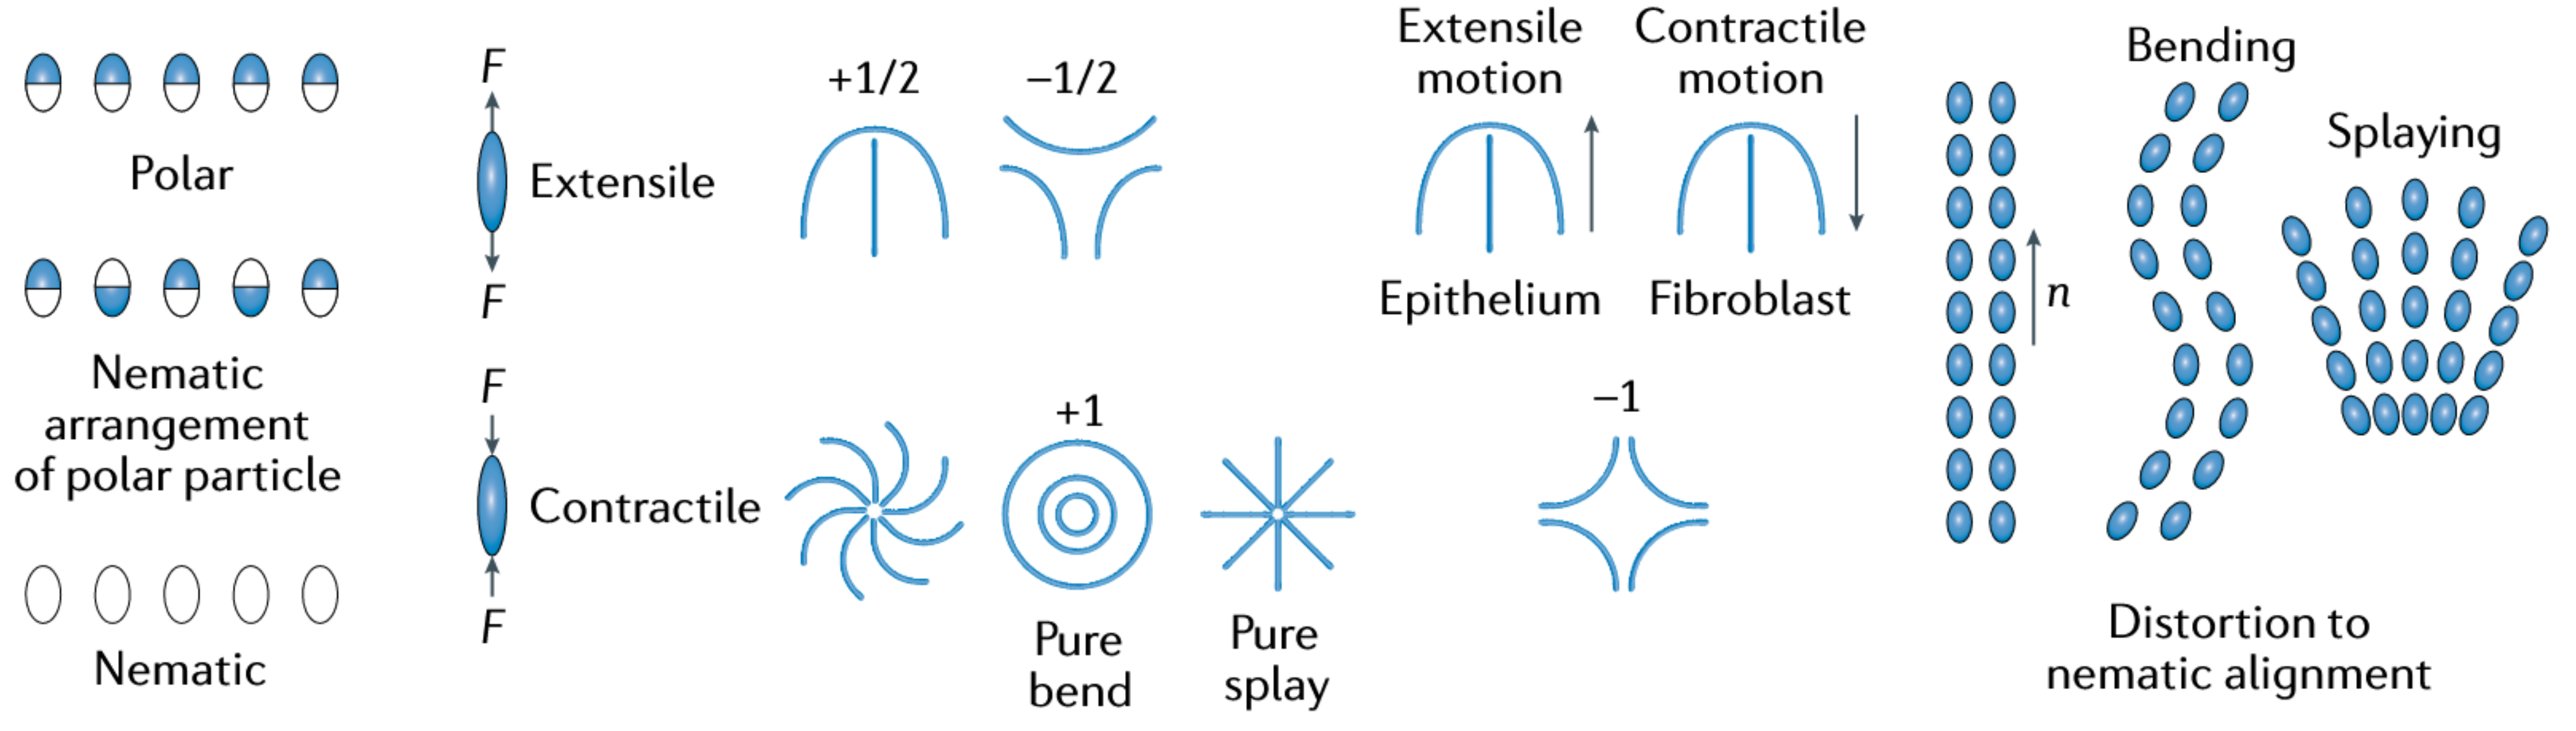
\includegraphics[width=\textwidth]{chap3nematic.png}
	\caption{\label{fig_3_10} \textbf{Active nematics}: Schematics of (A) nematic or polar particles, (B) extensile and contractile force dipoles, (C) Various types of defects and related motion of cells \textit{Adapted from \cite{xi2018}}. 
	}
\end{figure}

The utilization of this formulation is significant in characterizing the active forces produced by the network. The stress is separated into two components: active and passive. The passive stress arises from the viscoelasticity of the material and the bending, splaying, and twisting of the aligned elements. The active stress, on the other hand, is calculated by combining the strength of activity, represented by the parameter zeta, and the nematic order matrix. The sign of zeta determines the type of force dipole generated; a negative sign results in contraction of the system, while a positive sign leads to expansion along the nematic axis.

The active stress plays a crucial role in the motion of the system and can result in chaotic motion even in low Reynolds number systems, as evidenced in dense bacterial systems of \textit{Bacillus subtilis} where jet flows and turbulent patterns have been observed, as well as in expanding monolayers where independent vortices have been recorded \cite{wensink2012, blanch-mercader2018}. The nematic formulation have proven to be effective in capturing the physics of 2D confined systems and expanding systems (reviewed in \cite{saw2018}).

In the context of 3D models, active surfaces are used to describe the actomyosin cortex near cell membranes or epithelium in embryos \cite{salbreux2017}. This thin sheet of matter generates internal forces and torques that drive shape changes at the cellular or tissue level. The resulting three-dimensional structures can be conceptualized as curved, active two-dimensional surfaces. Forces and torques can be defined in terms of tension (\(t\)) and moment (\(m\)), and the model also considers the mirror and rotation symmetries of the surface elements (see Fig. \ref{fig_3_9}).
%
%\begin{figure}
%	\caption{\textbf{Active surface models}: (A) Tissues or cell surfaces can be modeled as surface with stresses and torques along the thickness. (B) Internal and external forces actin on a surface element. The kinematics of these surfaces, mathematical tools from differential geometry can be applied, using generalized coordinates ($\mathbf{X}$), metric tensor ($\mathbf{g}$), and curvature tensor ($\mathbf{C}$), where ($dl$) is the length of the line element with tangential unit vector ($v$). \textit{Adapted from \cite{salbreux2017}}}\label{fig_3_9}
%	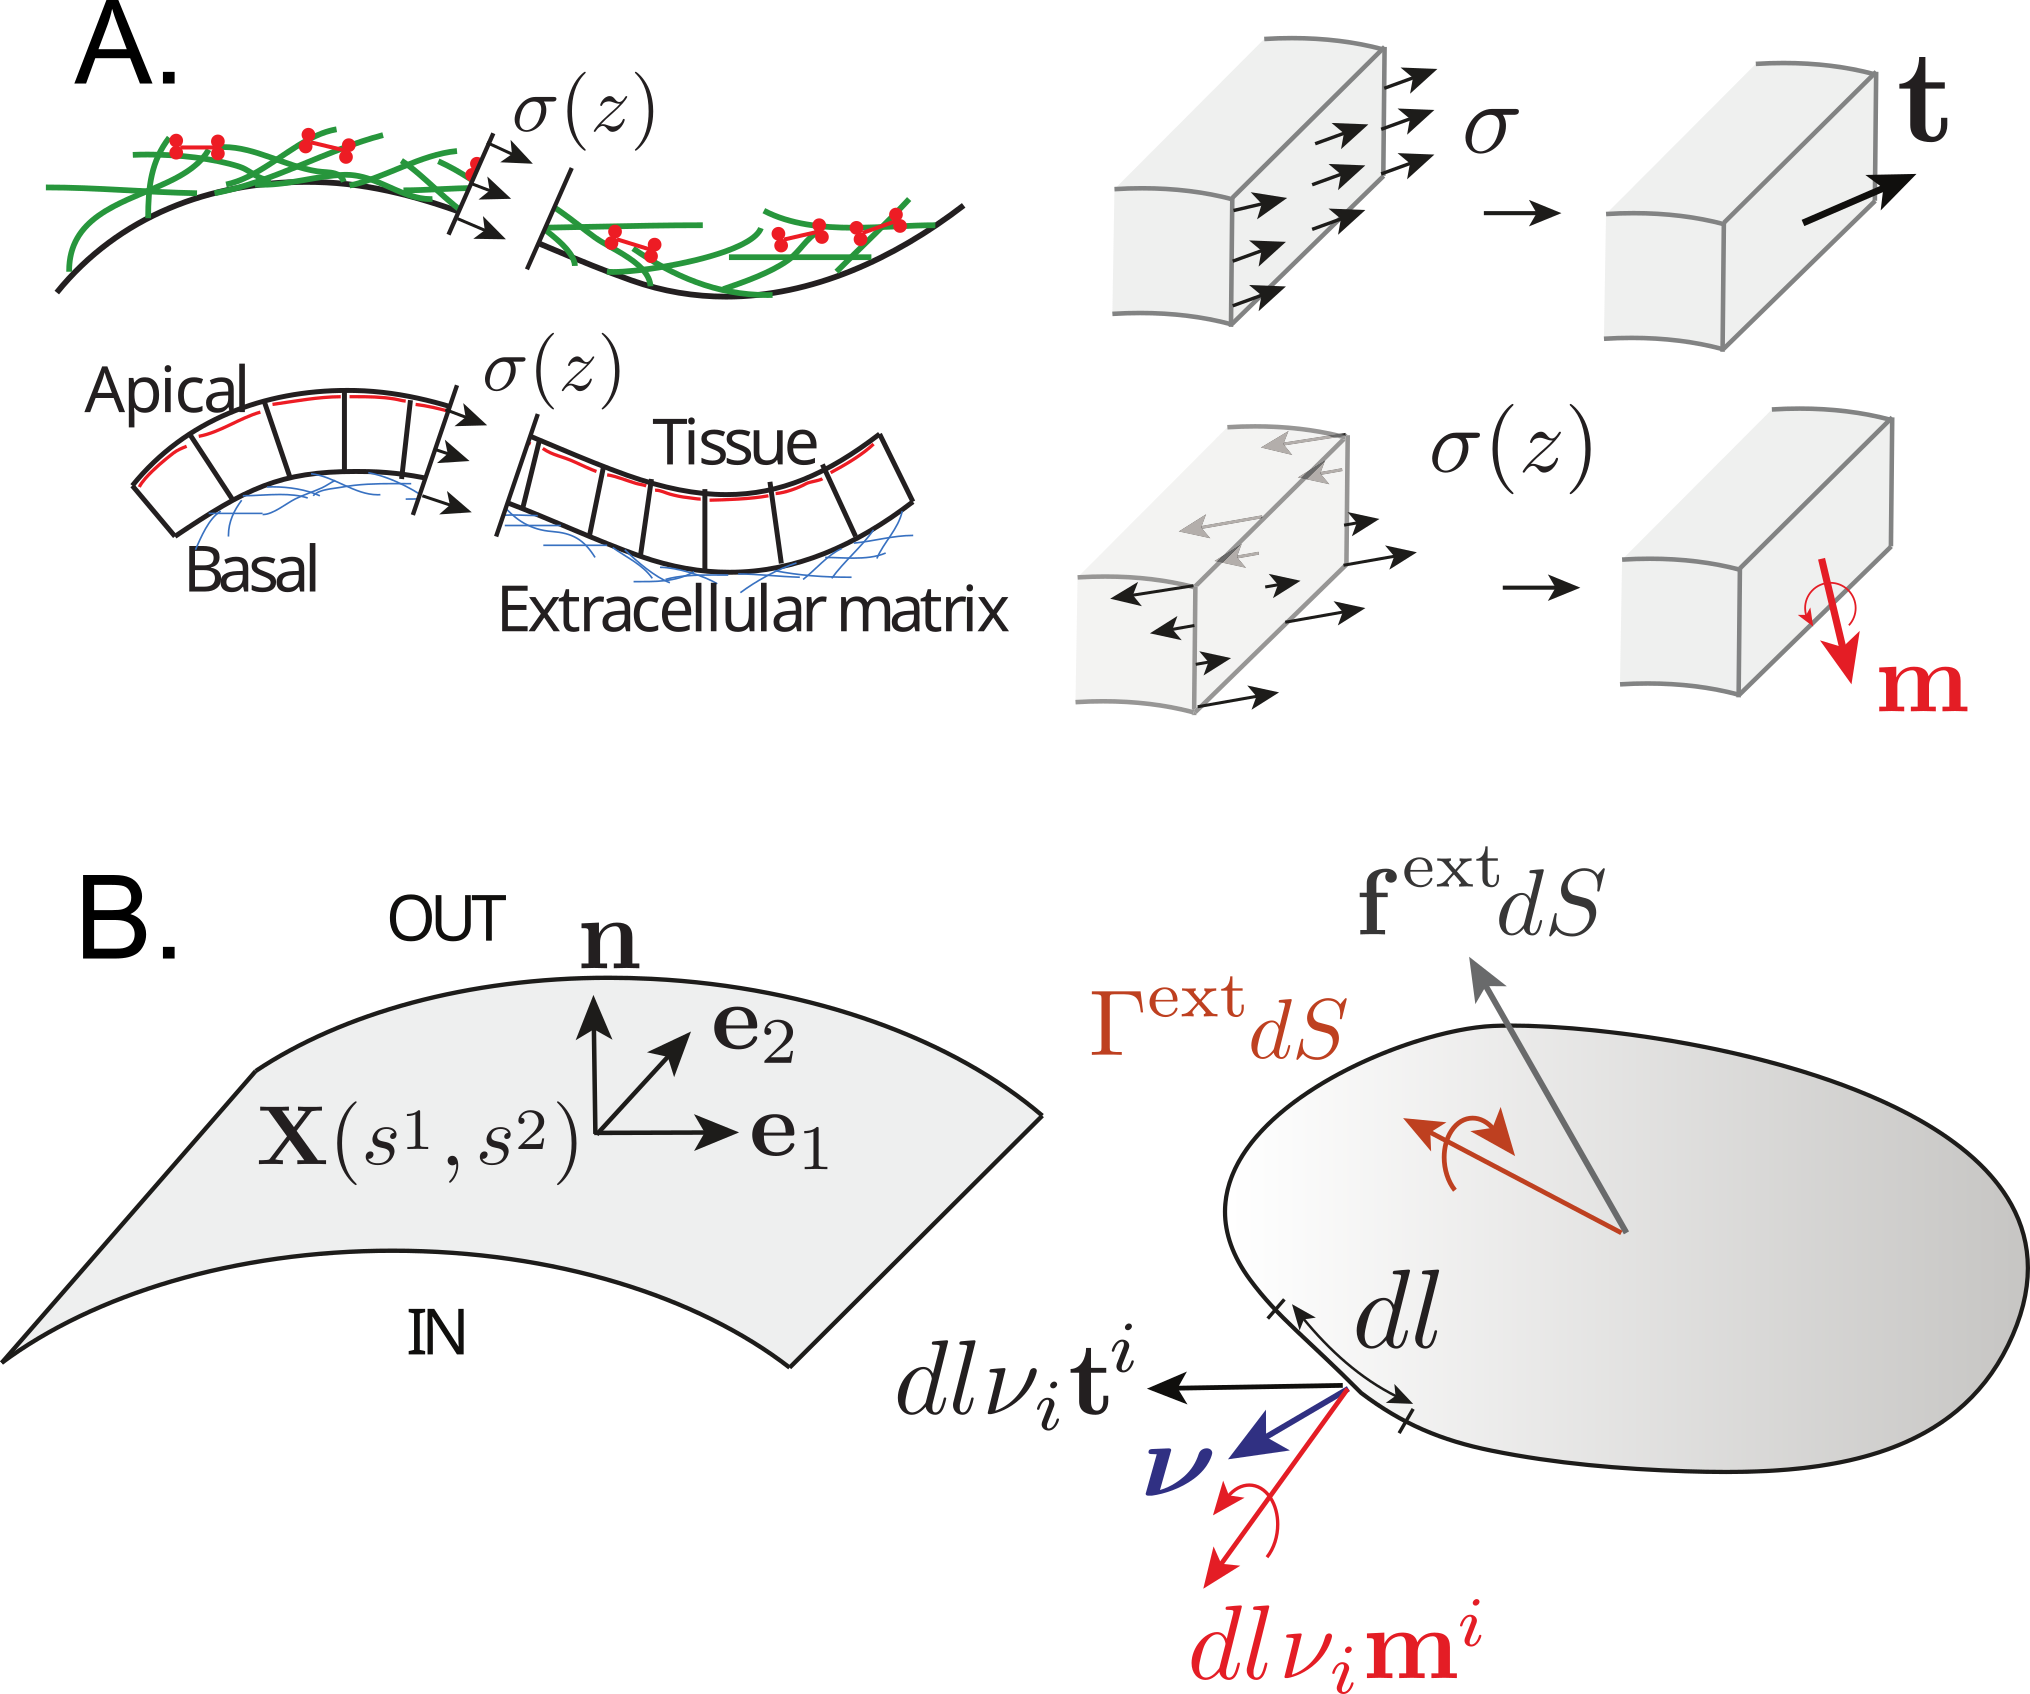
\includegraphics[width=7cm]{chap3activesurface.png}
%\end{figure} 
%

\begin{figure}
	\begin{minipage}[c]{0.5\textwidth}
		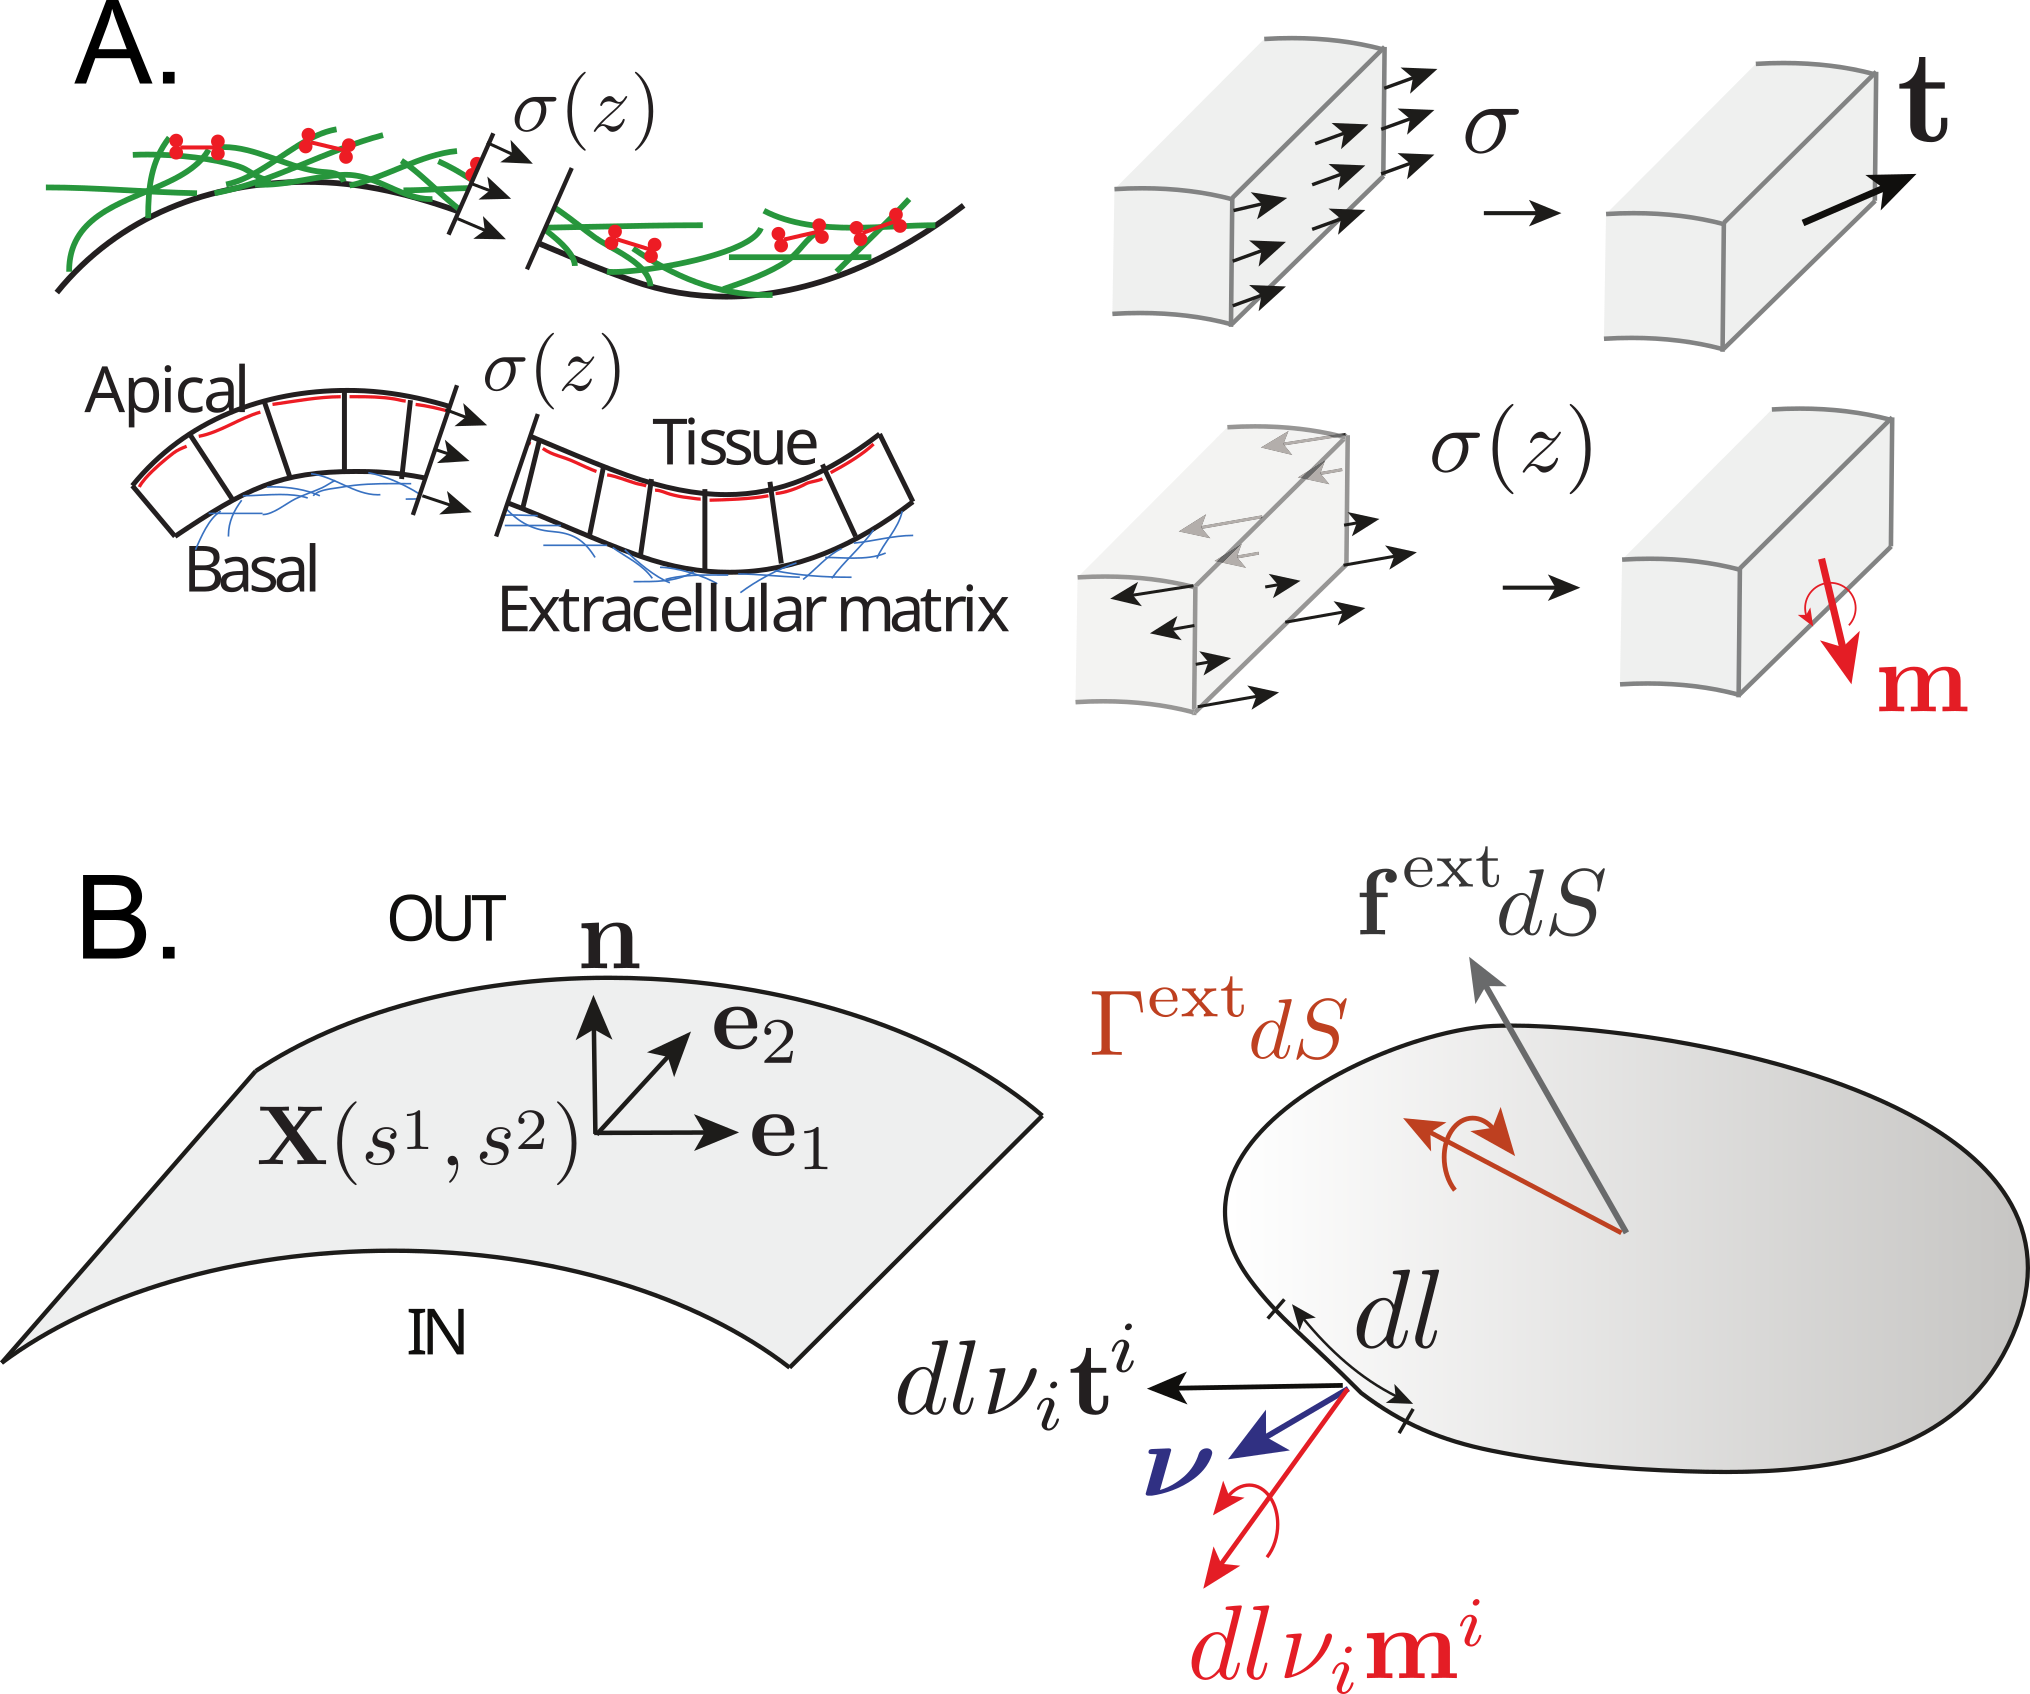
\includegraphics[width=\textwidth]{chap3activesurface.png}
	\end{minipage}\hfill
	\begin{minipage}[c]{0.45\textwidth}
		\caption{\textbf{Active surface models}: (A) Tissues or cell surfaces can be modeled as surface with stresses and torques along the thickness. (B) Internal and external forces actin on a surface element. The kinematics of these surfaces, mathematical tools from differential geometry can be applied, using generalized coordinates ($\mathbf{X}$), metric tensor ($\mathbf{g}$), and curvature tensor ($\mathbf{C}$), where ($dl$) is the length of the line element with tangential unit vector ($v$). \textit{Adapted from \cite{salbreux2017}}
		} \label{fig_3_9}
	\end{minipage}
\end{figure}





Salbreux and Julicher's work has demonstrated that flat active membranes with up-down asymmetry exhibit stability dependent on active tension and active tension-curvature coupling term. This tension-curvature dependency has been observed in the pancreas of mice, where the morphology of epithelial tumors is determined by the interplay of cytoskeletal changes in transformed cells and the existing tubular geometry \cite{messal2019}. Specifically, small pancreatic ducts produced exophytic growth, whereas large ducts deformed endophytically, consistent with theoretical predictions. Another example shows that curls of high curvature form spontaneously at the free edge of suspended epithelial monolayers, which originate from an enrichment of myosin in the basal domain that generates an active spontaneous curvature \cite{fouchard2020}. The extent of curling is controlled by the interplay between internal stresses in the monolayer.

While the molecular level behind epithelial morphogenesis, specifically the actin cytoskeleton, is well understood, there are still gaps in the theoretical and experimental framework that can bridge the gap between molecular dynamics and tissue-scale deformations. Vertex and continuum models have been developed to capture the physics of morphogenesis at the tissue scale, and phenomenological experiments provide insights into the constitutive relations of cytoskeletal components and tissues in specific conditions. However, combining vertex models and active surface mechanics could provide finer control over individual cell surfaces, enabling more precise bottom-up morphogenesis.